%TCIDATA{LaTeXparent=0,0,relatorio.tex}
\chapter{Resultados\label{chap:Resultados}}

\resumodocapitulo{Este capítulo apresenta resultados de simulação, os procedimentos experimentais realizados e seus resultados.}


\section{Câmera}

Os problemas com a câmera se resumiram à configuração da rede, à calibração e à programação. O mais difícil inicialmente foi a programação, mas se tornou bem simples depois.

\subsection{Configuração da Rede}
A câmera estava com um \textit{firmware} antigo e foi necessário obter o arquivo 2014R1B PresencePLUS Firmware\footnote{Atualização de Firmware da Câmera - \url{http://info.bannerengineering.com/_dav/cs/idcplg?IdcService=GET_FILE&RevisionSelectionMethod=LatestReleased&dDocName=B_4170042}. Acesso em 29/11/2015.} que é o programa de atualização da \textit{Banner Engineering} para esta câmera. Bastou executá-lo no computador, estando a câmera conectada ao \textit{switch} do laboratório assim como o computador estava, ambos por cabos Ethernet. Antes desta atualização, o \textit{software} da câmera não permitia selecionar a opção Ethernet/IP de forma a permitir utilizar o módulo Ethernet/IP do CLP.

Uma vez atualizado o \textit{firmware}, foi obtido o arquivo EDS\footnote{Arquivo EDS disponível em \url{http://www.bannerengineering.com/en-US/products/sub/78\#ui-tabs-37}. Acesso em 29/11/2015.} da câmera que foi então integrado ao \textit{software} da Rockwell no computador por meio do programa \textit{EDS Hardware Installation Tool} da própria Rockwell, parte do RSLinx.

Após os procedimentos anteriores, adiciona-se a câmera como um módulo genérico usando o \textit{software} RSLogix, conforme instruções da Banner Engineering \cite{presencePlusEthernetIP}. Foi também necessário utilizar o RSLinx para verificar se a câmera  estava conectada ao computador e o \textit{software} da PresencePlus para identificar a câmera pelo endereço IP, uma vez que a rede utilizada é Ethernet/IP. A Figura \ref{linxcamera} mostra a janela do RSLinx com a câmera reconhecida.

\begin{figure}[!ht]
\centering
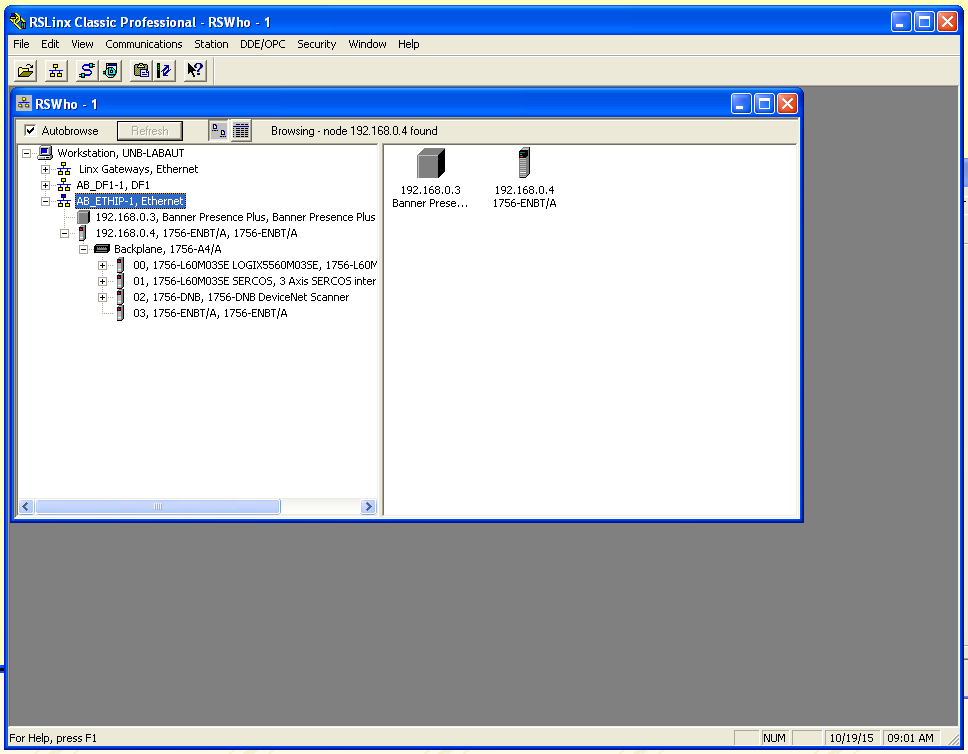
\includegraphics[width=\linewidth]{figs/resultados/camera/cameralinx}
\caption{RSLinx com câmera reconhecida \label{linxcamera}}
\end{figure}

\subsection{Calibração}

A câmera permite fazer medidas de distâncias em \textit{pixels}. De forma a se converter essa distância para milímetros, uma barra de alumínio com marcas e tamanho conhecido é utilizada. É importante primeiro calibrar o sistema, para se saber se há deformação de pixels significante ao longo da distância de interesse, nomeadamente o tamanho da barra de alumínio sendo utilizada, cerca de $532$mm. No PresencePlus P4 GEO 1.3, um programa é feito, com imagem de referência conforme Figura \ref{cameracalibracao}, que usa várias ferramentas de detecção de borda (ferramenta \texttt{Locate}) para identificar as posições de cada uma das marcas pretas da barra. Seis marcas foram feitas e a Tabela \ref{relacoesmmpx} apresenta os resultados para cada seção. A distância entre duas marcas é de 10cm, com exceção da distância entre P0 e PEND que é o comprimento total da barra.

\begin{figure}[!ht]
\centering
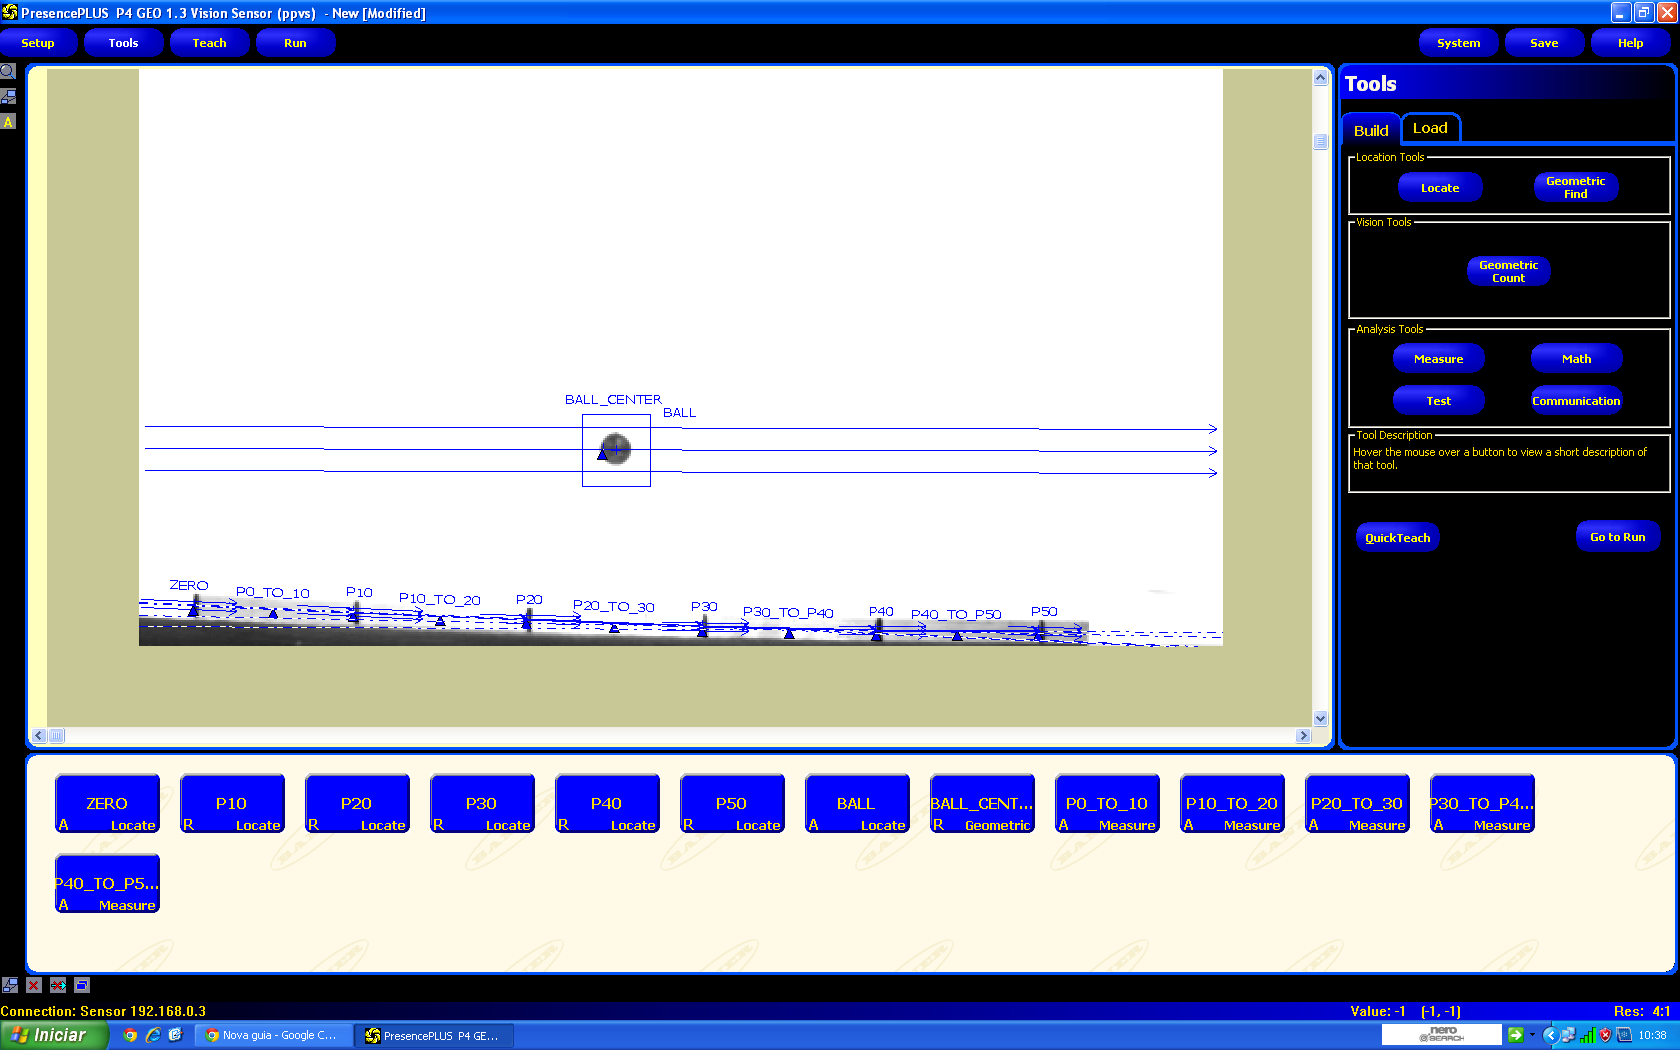
\includegraphics[width=0.9\linewidth]{figs/resultados/camera/programa}
\caption{Programa PresencePLUS para calibração da câmera \label{cameracalibracao}}
\end{figure}

\begin{table}[!ht]
\centering
\caption{Relações mm/px para diferentes seções da barra de alumínio \label{relacoesmmpx}}
	\begin{tabular}{|c|c|c|c|}
	\hline
		Seção 1 & Seção 2 & Distância (px) & mm/px\\ \hline
		P0 & P10 & 160 & 0.625\\ \hline
		P10 & P20 & 173 & 0.578\\ \hline
		P20 & P30 & 176 & 0.568\\ \hline
		P30 & P40 & 173 & 0.578\\ \hline
		P40 & P50 & 163 & 0.613\\ \hline
		P0 & PEND & 893 & 0.596\\ \hline
	\end{tabular}
\end{table}

O maior desvio da quantidade de milímetros por \textit{pixel} das seções em relação à da barra inteira é de aproximadamente 4.93\%. Há algumas imprecisões na maneira como os traços foram desenhados e é possível que o erro seja menor.

\subsection{Programação}
A programação da câmera se inicia obtendo uma imagem de referência e adicionando-se ferramentas de detecção de pontos de interesse, como mostra a Figura \ref{cameracalibracao}. A ferramenta \texttt{Locate} é responsável por detectar as bordas da bolinha, e a ferramenta \texttt{Geometric} detecta o centro da mesma. Também é possível adicionar ferramentas que fazem operações matemáticas (ferramenta \texttt{Math}), executam medições (ferramenta \texttt{Measure}), assim como as que enviam dados pela rede (ferramenta \texttt{Communication}), o que é essencial para se comunicar com o CLP.

\section{Calibração do Servomotor\label{calibracaoServomotorSecao}}

O RSLogix tem o bloco \texttt{MAJ} \textendash{} \textit{Motion Axis Jog} \textendash{} que permite alterar a velocidade do motor enquanto ele se movimenta. No entanto, o bloco espera que a entrada tenha unidade $[\mathrm{u}/\mathrm{s}]$ (unidades por segundo) ao invés de alguma unidade no SI tal como $[\mathrm{mm}/\mathrm{s}]$. Devido a isso, foi necessária uma calibração do sistema. O procedimento era anotar a posição inicial $x_0$, definir um tempo $\Delta t$ no qual o carrinho se movimenta a uma velocidade $v$ em $[\mathrm{u}/\mathrm{s}]$ e, após o movimento,  registrar a posição final $x_f$. As posições inicial e final são medidas em milímetros. Com isso, calculava-se a velocidade em $[\mathrm{mm}/\mathrm{s}]$. Alguns ensaios são realizados seguindo esse procedimento e a média é considerada como o valor de uma unidade, resultando em aproximadamente $71.32\mathrm{mm}$. Os dados de calibração estão na Tabela \ref{calibracaoServomotor}.

\begin{table}[!ht]
\centering
\caption{Dados de calibração do servomotor, média obtida é de 71.32 mm/unidade\label{calibracaoServomotor}}
\begin{tabular}{|c|c|c|c|c|c|}
\hline
	$x_0$ - [mm] & $x_f$ - [mm] & $\Delta t$ - [s] & Velocidade - [u/s] & Velocidade - [mm/s] & mm/u\\ \hline
2 &	71.8  &	2   &	0.5 &	34.9   & 	69.8\\ \hline
6 & 76.1  &	2   &	0.5 &	35.05  &	70.1\\ \hline
6 &	188	  &  5   &	0.5	&   36.4   &	72.8\\ \hline
6 &	185   &	2.5 &	1	& 	71.6   &	71.6\\ \hline
6 &	77    &	10  &	0.1	&   7.1    &	71\\ \hline
6 &	296.5 &	20	&   0.2 & 	14.525 &	72.625\\ \hline\end{tabular}
\end{table}

\section{Modelo no Espaço de Estados}

A partir da teoria apresentada na Subseção \ref{reducaoModal}, foram desenvolvidas algumas rotinas em linguagem Julia \cite{julia} para obtenção das matrizes reduzidas. Na rotina, a ordem da matriz de saída é um parâmetro, mas para os propósitos deste projeto só foi testado o sistema reduzido a quatro estados. A Seção \ref{reducaoModalPrograma} dos anexos apresenta o código completo.

As matrizes obtidas para o modelo reduzido são dadas \begin{align}
\begin{array}{ll}
	\mathbf{A_R} &= \left[\begin{array}{cccc}
		-0.0881  & -3.8389 &         0 &         0\\
    3.8389 &   -0.0881 &         0 &         0\\
         0 &         0 &   -0.1061 &  -10.8145\\
         0 &        0 &   10.8145 &   -0.1061\\
	\end{array}\right],\\
	\mathbf{B_R} &= 10^3\left[0.3313,\;
    0.0066,\;
    1.3549,\;
    0.0163\right]^{\mathrm{T}},\\
	\mathbf{C_R} &= \left[-0.0003,\;0.0148,\;0.0001,\;-0.0029\right]\;\mathrm{e}\\
	D_R &= -0.0906,
\end{array} \label{modeloReduzidoSemEpsilon}
\end{align} sendo que é fácil observar que os autovalores da matriz $\mathbf{A_R}$ são dados por $-0.0881\pm 3.8389j$ e $-0.1061\pm 10.8145j$, valores extraídos dos blocos diagonais dessa matriz. Esse tipo de estrutura já era esperada quando se apresentou a técnica de redução modal na subseção \ref{reducaoModal}. O sistema composto por essas matrizes é dado por \begin{align}
	\begin{array}{ll}
		\mathbf{\dot{z}} &= \mathbf{A_R}\mathbf{z} + \mathbf{B_R}u(t)\;\mathrm{e}\\
		y &= \mathbf{C_R}\mathbf{z} + D_Ru(t).
	\end{array}\label{modeloEspacoDeEstadosSemAtraso}
\end{align}


No sistema da Equação \ref{modeloEspacoDeEstadosSemAtraso}, ainda não se compensou pela transferência direta diferente de zero. Note que ela era zero antes da redução, mas a perca do ganho estático dos outros modos do sistema levou a esse $D_R$ não nulo. Quando se analisa a resposta ao degrau em malha aberta para este caso, Figura \ref{modeloMalhaAberta}, nota-se que o atraso é cerca de 0.3s. Para ser preciso, $\epsilon = 0.313$s. Com esse valor de atraso, calculam-se novas matrizes $\mathrm{B}_D$ e $D_D$ para substituir $\mathrm{B}_R$ e $D_R$, respectivamente, conforme Equações \ref{novoBD} e \ref{novoDD}. Utilizando exatamente esse atraso de $0.313$s, a transferência direta se tornaria aproximadamente zero. No entanto, esses modelos no espaço contínuo serão discretizados com período $T_s = 0.1$s. Daí, o $\epsilon$ mais próximo realizável é 0.3s e seu uso resulta nas novas matrizes \begin{align}
\begin{array}{ll}
	\mathbf{B_D} &= 10^3\left[0.1255,\;
    0.2974,\;
   -1.3039,\;
   -0.1504\right]^{\mathrm{T}}\;\mathrm{e}\\
	D_D &= -0.0685,
\end{array} \label{modeloReduzidoComEpsilon}
\end{align} que então fazem parte do novo sistema reduzido dado por\begin{align}
	\begin{array}{ll}
		\mathbf{\dot{z}} &= \mathbf{A_R}\mathbf{z} + \mathbf{B_D}u(t-\epsilon)\;\mathrm{e}\\
		y &= \mathbf{C_R}\mathbf{z} + D_D u(t-\epsilon).
	\end{array}\label{modeloEEComAtraso}
\end{align}

\begin{figure}[!ht]
\centering
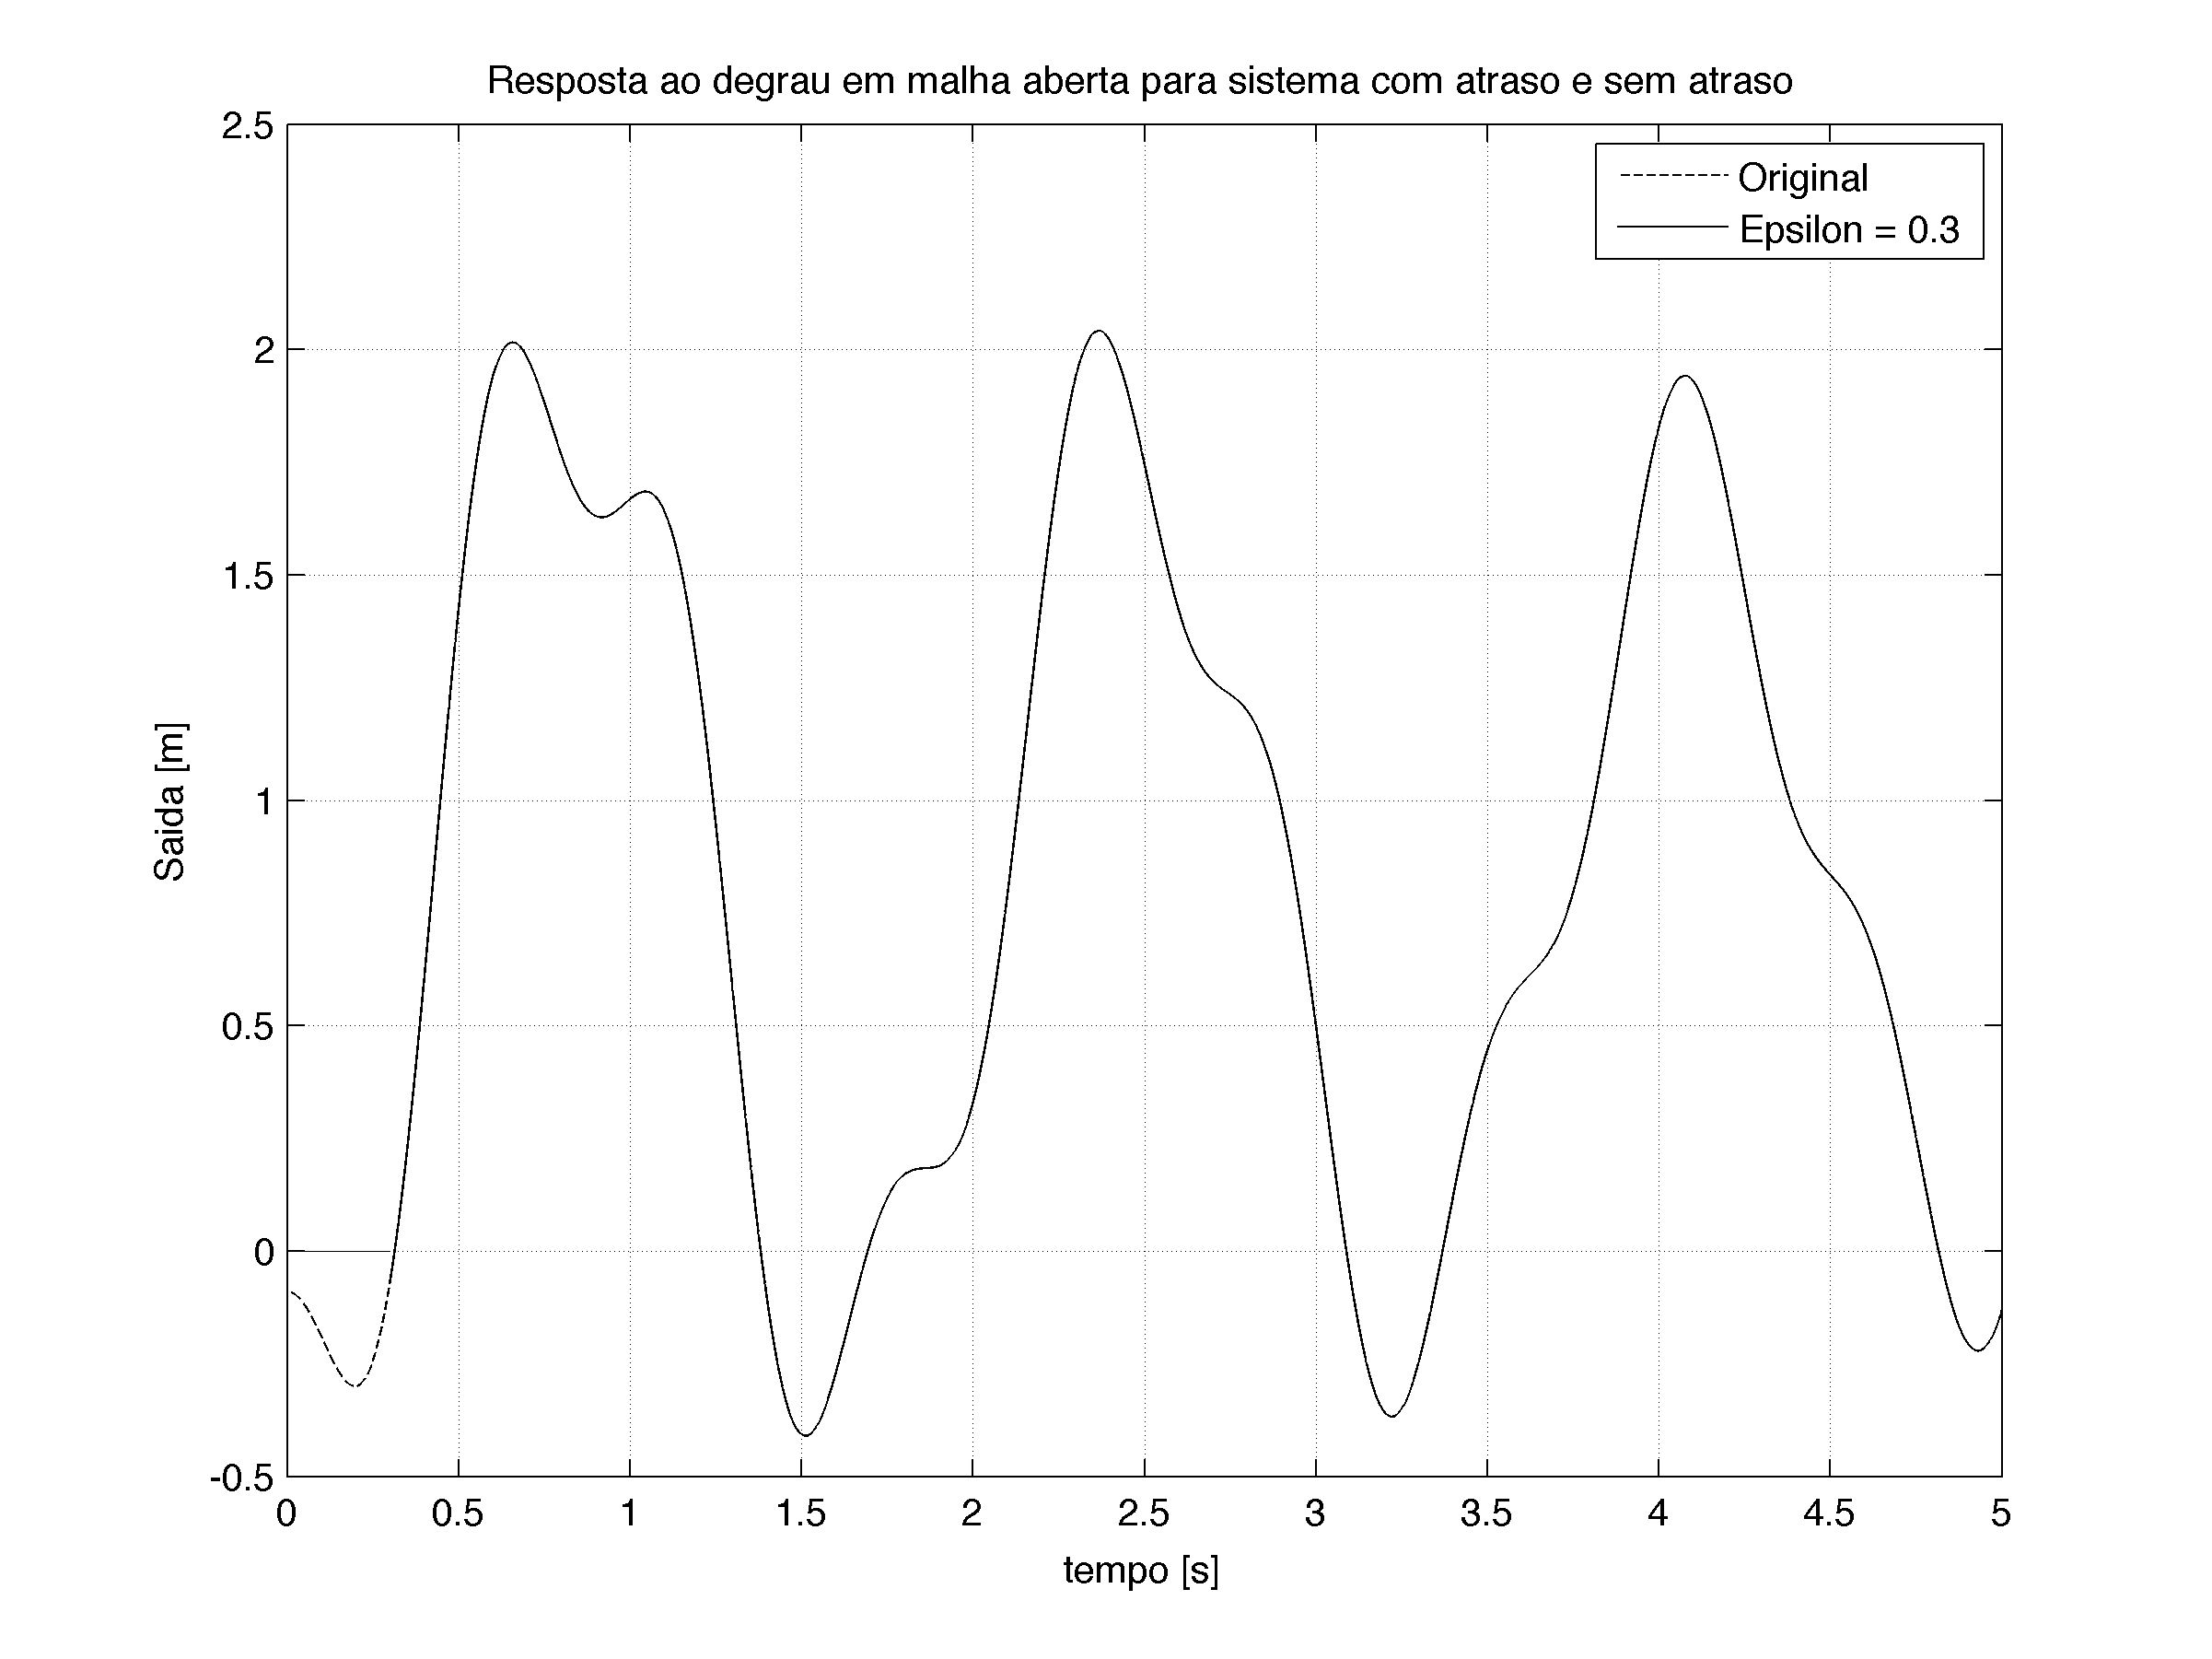
\includegraphics[width=0.8\linewidth]{figs/resultados/modelo/respostaMalhaAberta}
\caption{Resposta ao degrau para modelos reduzidos com atraso e sem atraso\label{modeloMalhaAberta}}
\end{figure} 

Apesar de $\epsilon=0.3$s ser próximo de 0.313s, esse atraso não reduz muito a transferência direta, como se pode observar analisando $D_D$, Equação \ref{modeloReduzidoComEpsilon}.



 O sistema em malha aberta oscila muito, mas é estável. Observa-se que a resposta decai conforme o tempo passa, conforme Figura \ref{modeloMalhaAberta25s}. O objetivo do controle é reduzir ao máximo essas oscilações, tendo uma trajetória o mais suave possível de um ponto inicial a um ponto final. 
\begin{figure}[!ht]
\centering

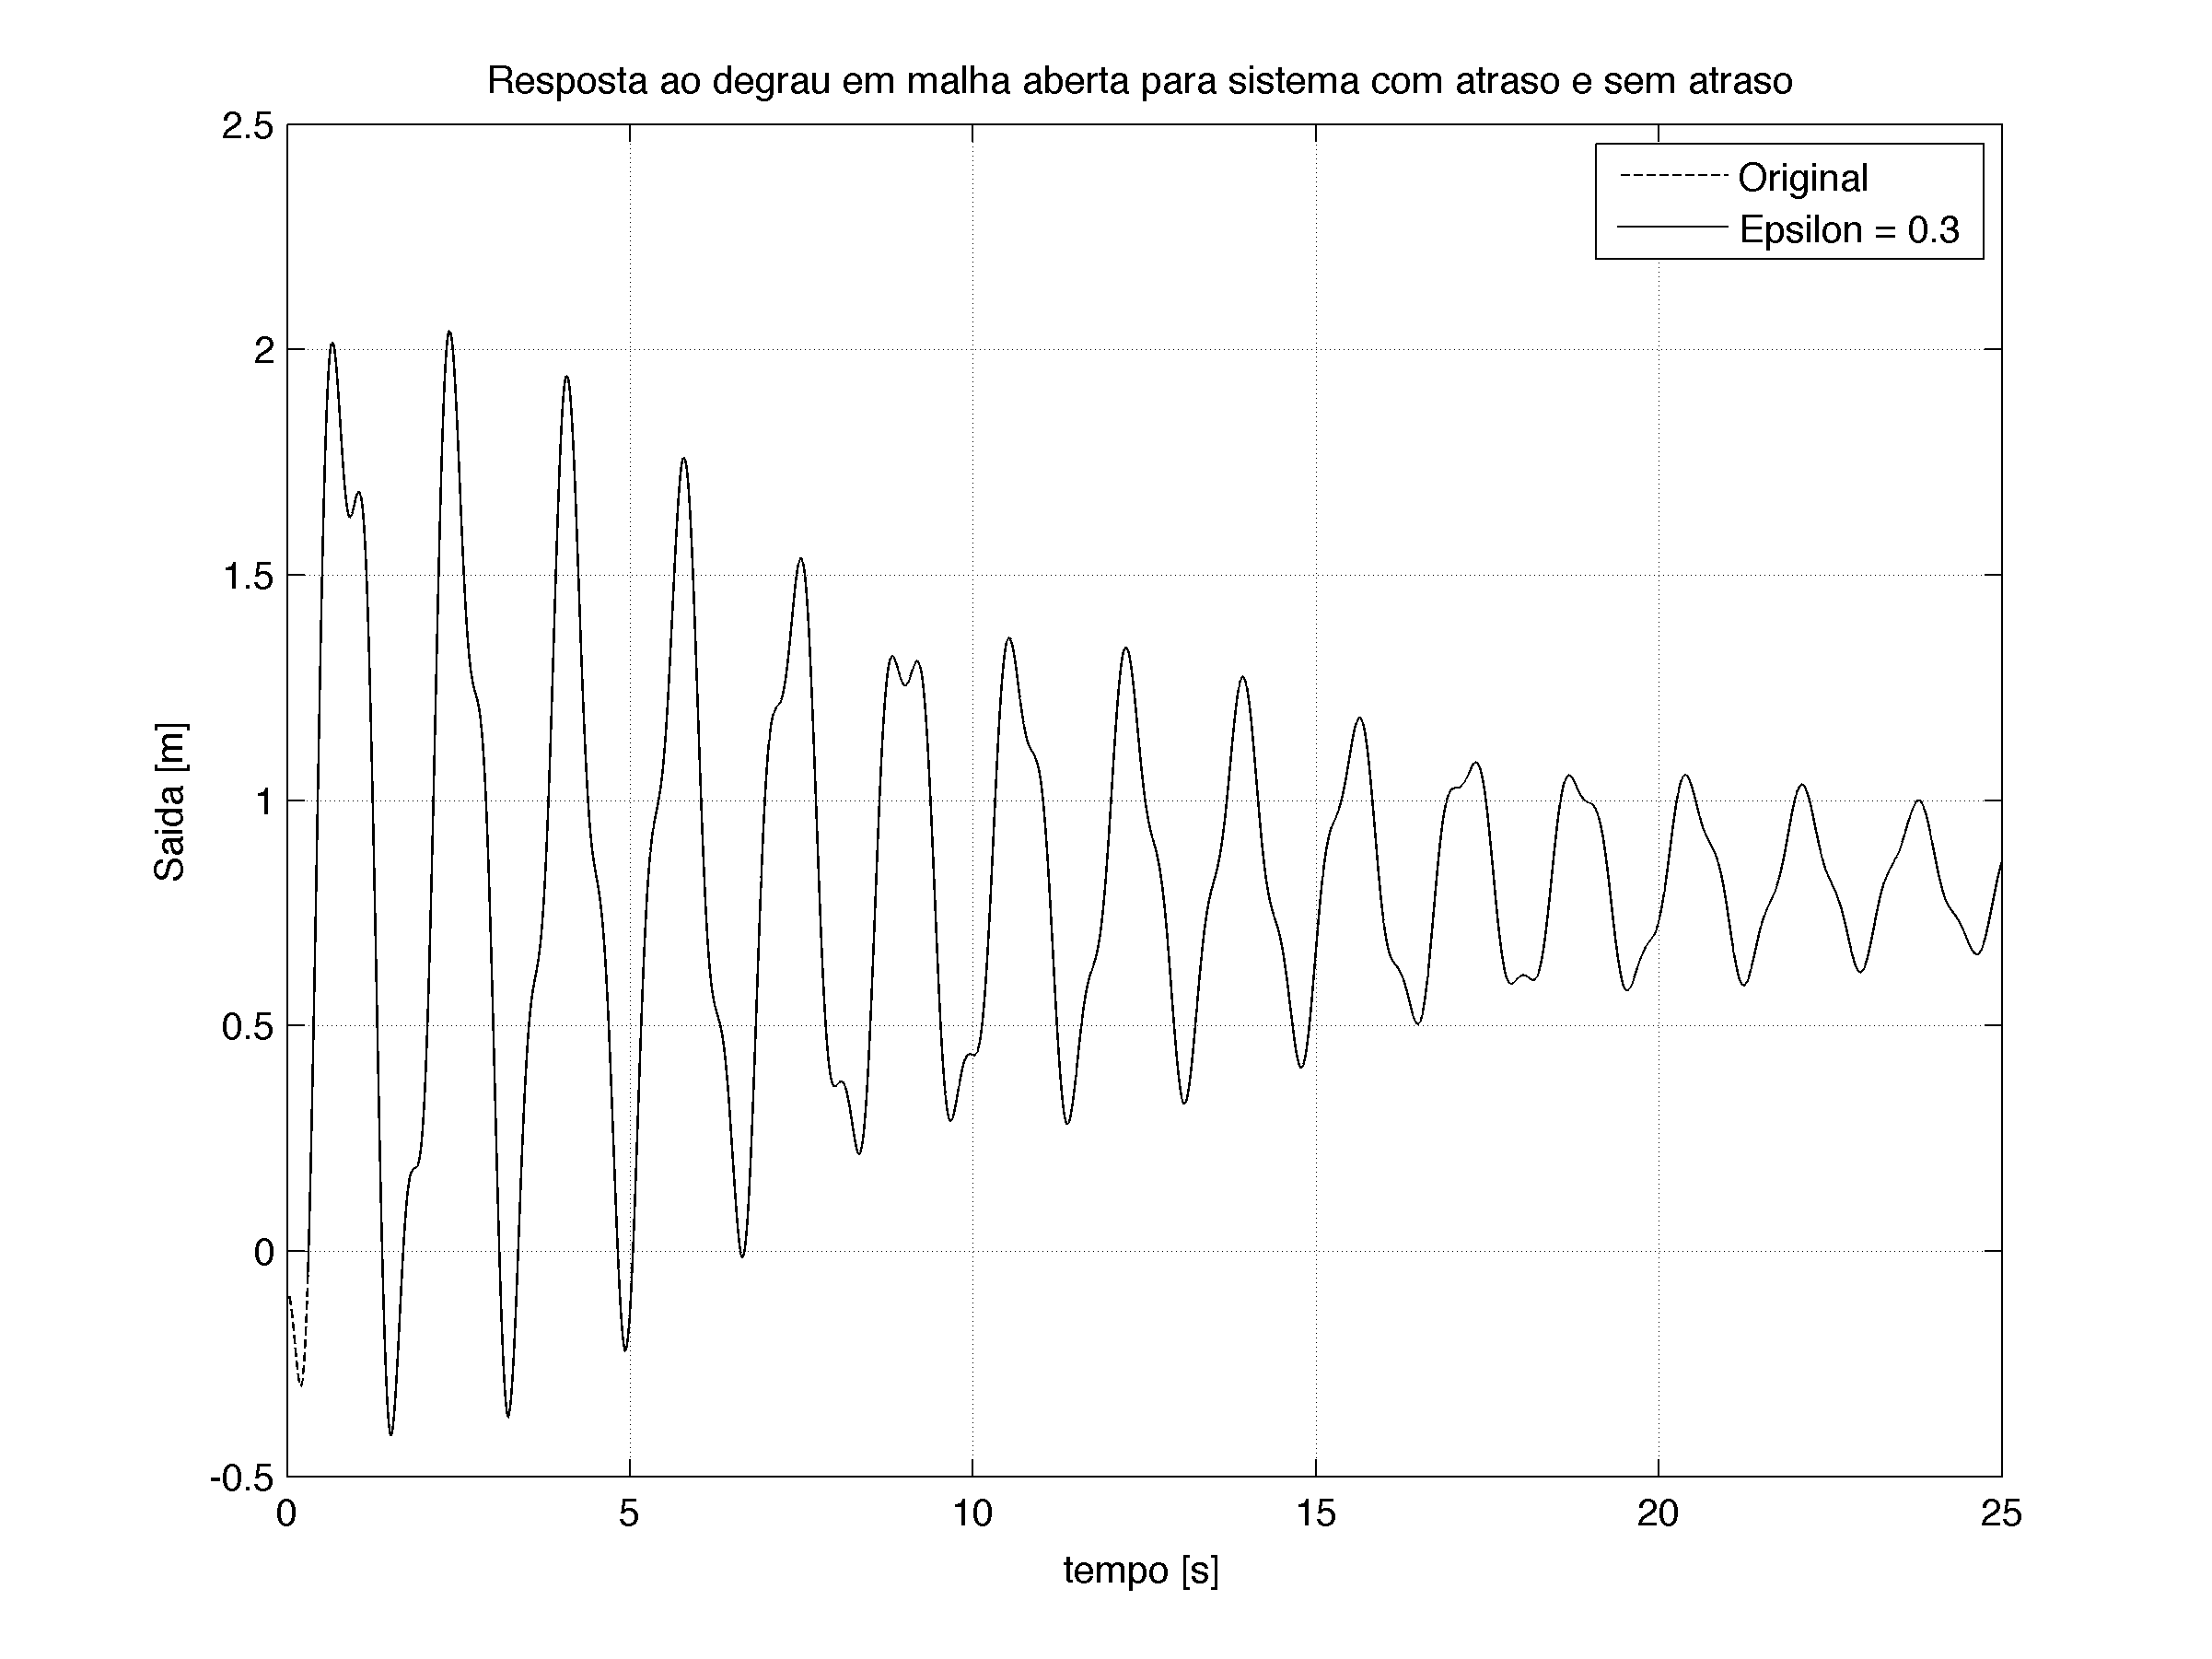
\includegraphics[width=0.8\linewidth]{figs/resultados/modelo/respostaMalhaAberta25s}
\caption{Resposta ao degrau para modelos reduzidos com atraso e sem atraso, 25 segundos\label{modeloMalhaAberta25s}}
\end{figure}

\subsection{Discretização}
 O controle será feito conforme a Seção \ref{controle}, mas primeiro deve-se discretizar o sistema.  A função \texttt{c2d} \cite{c2d} do MATLAB é utilizada, resultando nas matrizes \begin{align}
 \begin{array}{ll}
 	\mathbf{A} &= \left[\begin{array}{cccc}
	0.9191&   -0.3712&         0&         0\\
    0.3712&    0.9191&         0&         0\\
         0&         0&    0.4651&   -0.8733\\
         0&         0&    0.8733&    0.4651\\
 \end{array}\right],\\
 	\mathbf{B} &= \left[6.5818,\;
   31.2517,\;
  -98.5991,\;
  -75.6695\right]^{\mathrm{T}},\\
   \mathbf{C} &= \left[-0.0003,\;0.0148,\;0.0001,\;-0.0029\right],\\
   D &= -0.0685.
 \end{array}
 \end{align}
 
 Os polos de $\mathbf{A}$ são $0.9191 \pm 0.3712j$ e $
   0.4651 \pm 0.8733j$. Como esses polos estão dentro do círculo unitário, o sistema continua estável, apesar de manter as oscilações, pelo fato dos polos terem parte imaginária. Vale notar que as matrizes $\mathbf{C}$ e $D$ são iguais a $\mathbf{C_R}$ e $D_D$ do sistema contínuo, respectivamente, conforme Equações \ref{modeloReduzidoSemEpsilon} e \ref{modeloReduzidoComEpsilon}.
 
\subsection{Controle}

 A parte mais difícil do controle é a escolha dos polos. Algumas simulações foram realizadas e observava-se se o sistema era estável e se oscilava muito. O projeto final considerou 5 polos: $\left[0.6,\;0.6,\;0.6,\;0.5\pm 0.4j\right]$. O primeiro polo se deve ao integrador que foi adicionado ao sistema. Os polos com parte imaginaria foram escolhidos baseados nos polos originais do sistema. A ideia é evitar forçar muito esses polos para longe, evitando que os ganhos sejam altos e economizando em atuação. Os ganhos obtidos para esse caso são dados por \begin{align}
 \begin{array}{ll}
	 	\mathbf{K_p} &= \left[0.0080,\;0.0096,\;-0.0046,\;-0.0004\right],\\
 	K_i &= 0.1953.\\ 	
 \end{array}\label{ganhosObtidos}
 \end{align}
 
 O código para calcular os ganhos está disponível na Seção \ref{projetoControlador}.

\section{Simulação}

 Antes de se implementar o controle na planta, é essencial a realização de simulações. Elas são rápidas de serem realizadas e permitem averiguar se um projeto é estável ou não. As simulações aqui realizadas incluem o sistema em malha aberta com entrada tipo rampa e a entrada suave, utilizada por \cite{rafaelMestrado}. Depois da apresentação dos resultados em malha aberta, são apresentados os resultados em malha fechada sem considerar ruído. Por fim, os resultados com um ruído somado são apresentados.
 
 O resultado da simulação em malha aberta é apresentado nas Figuras \ref{respostaMalhaAbertaRampa} e \ref{respostaMalhaAbertaEntradaSuave}. Nota-se que a resposta à rampa teve diversas oscilações que demoram a atenuar-se. Já a entrada calculada por \cite{rafaelMestrado} teve uma ótima resposta. A desvantagem da implementação em malha aberta é que ela não resiste a perturbações e essas sempre ocorrem, ainda mais quando se considera o fundo do oceano.
 
 \begin{figure}[!htb]
    \centering
    \begin{minipage}{.45\textwidth}
        \centering
        
        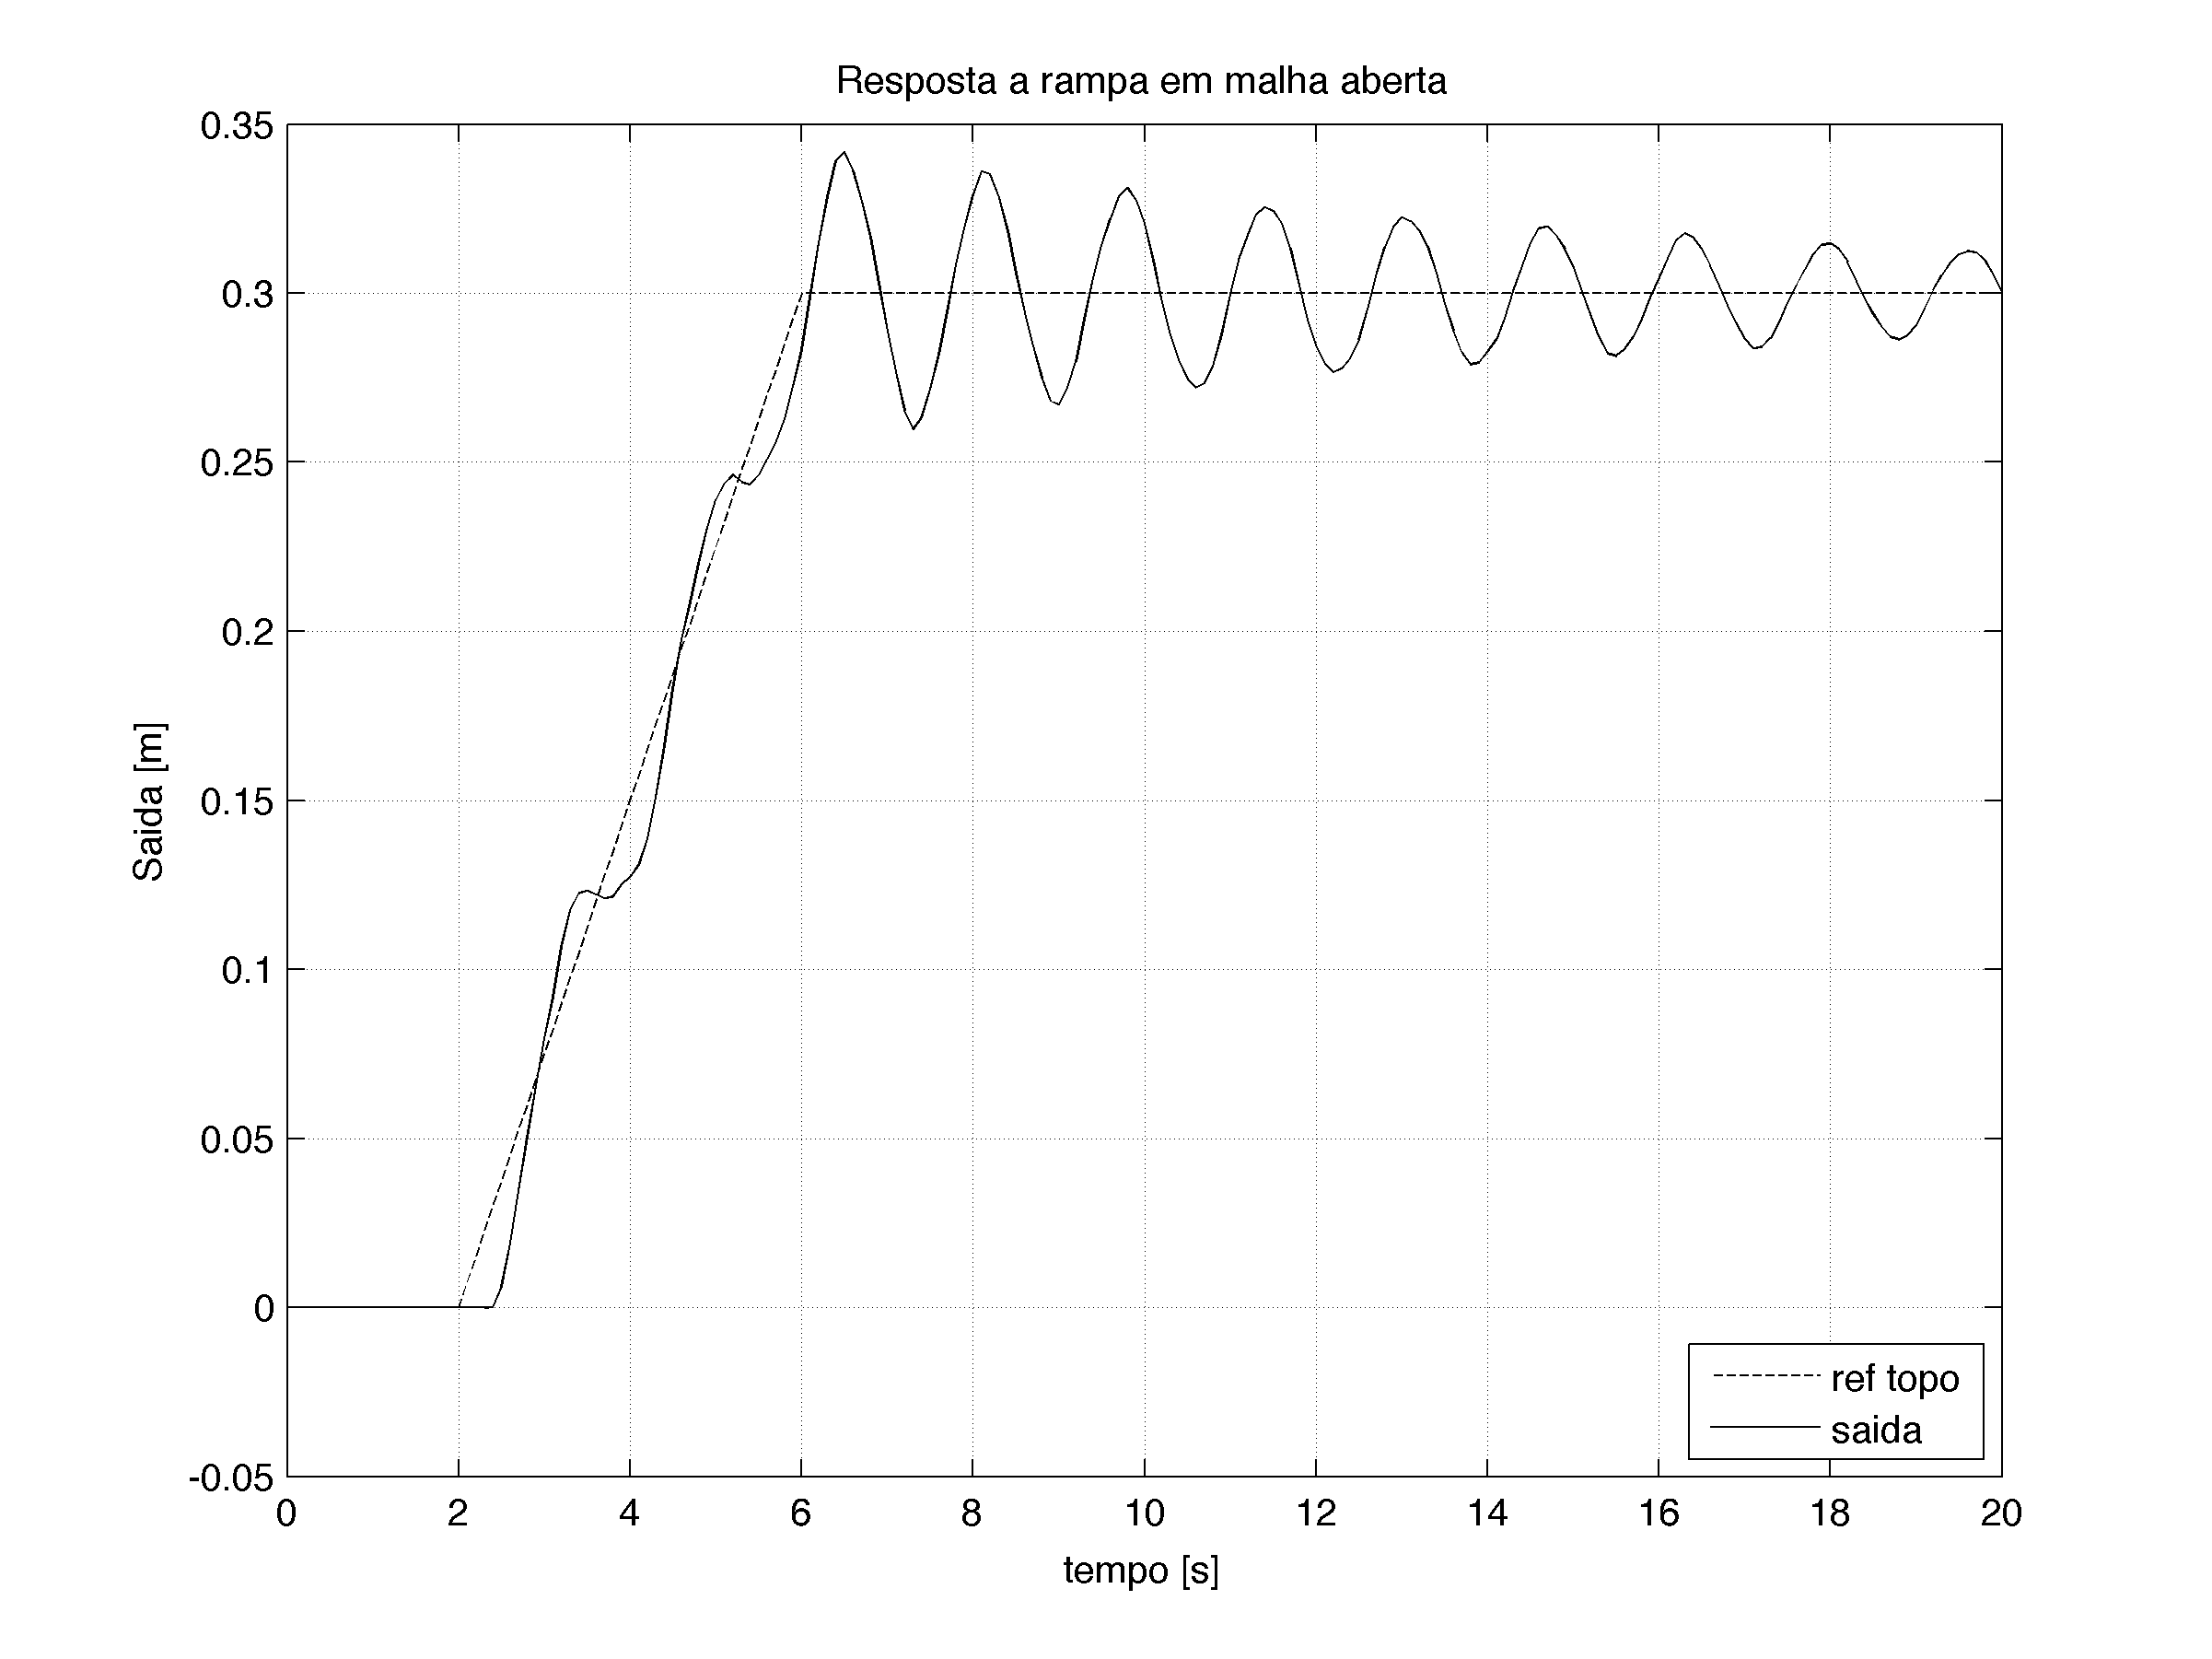
\includegraphics[width=1\linewidth]{figs/resultados/simulacao/respostaMalhaAbertaRampa}
        \caption{Resposta do Sistema em Malha Aberta para Excursão de 30cm, entrada rampa\label{respostaMalhaAbertaRampa}}
    \end{minipage}%
    \hspace{0.1cm}
    \begin{minipage}{0.45\textwidth}
        \centering
        
        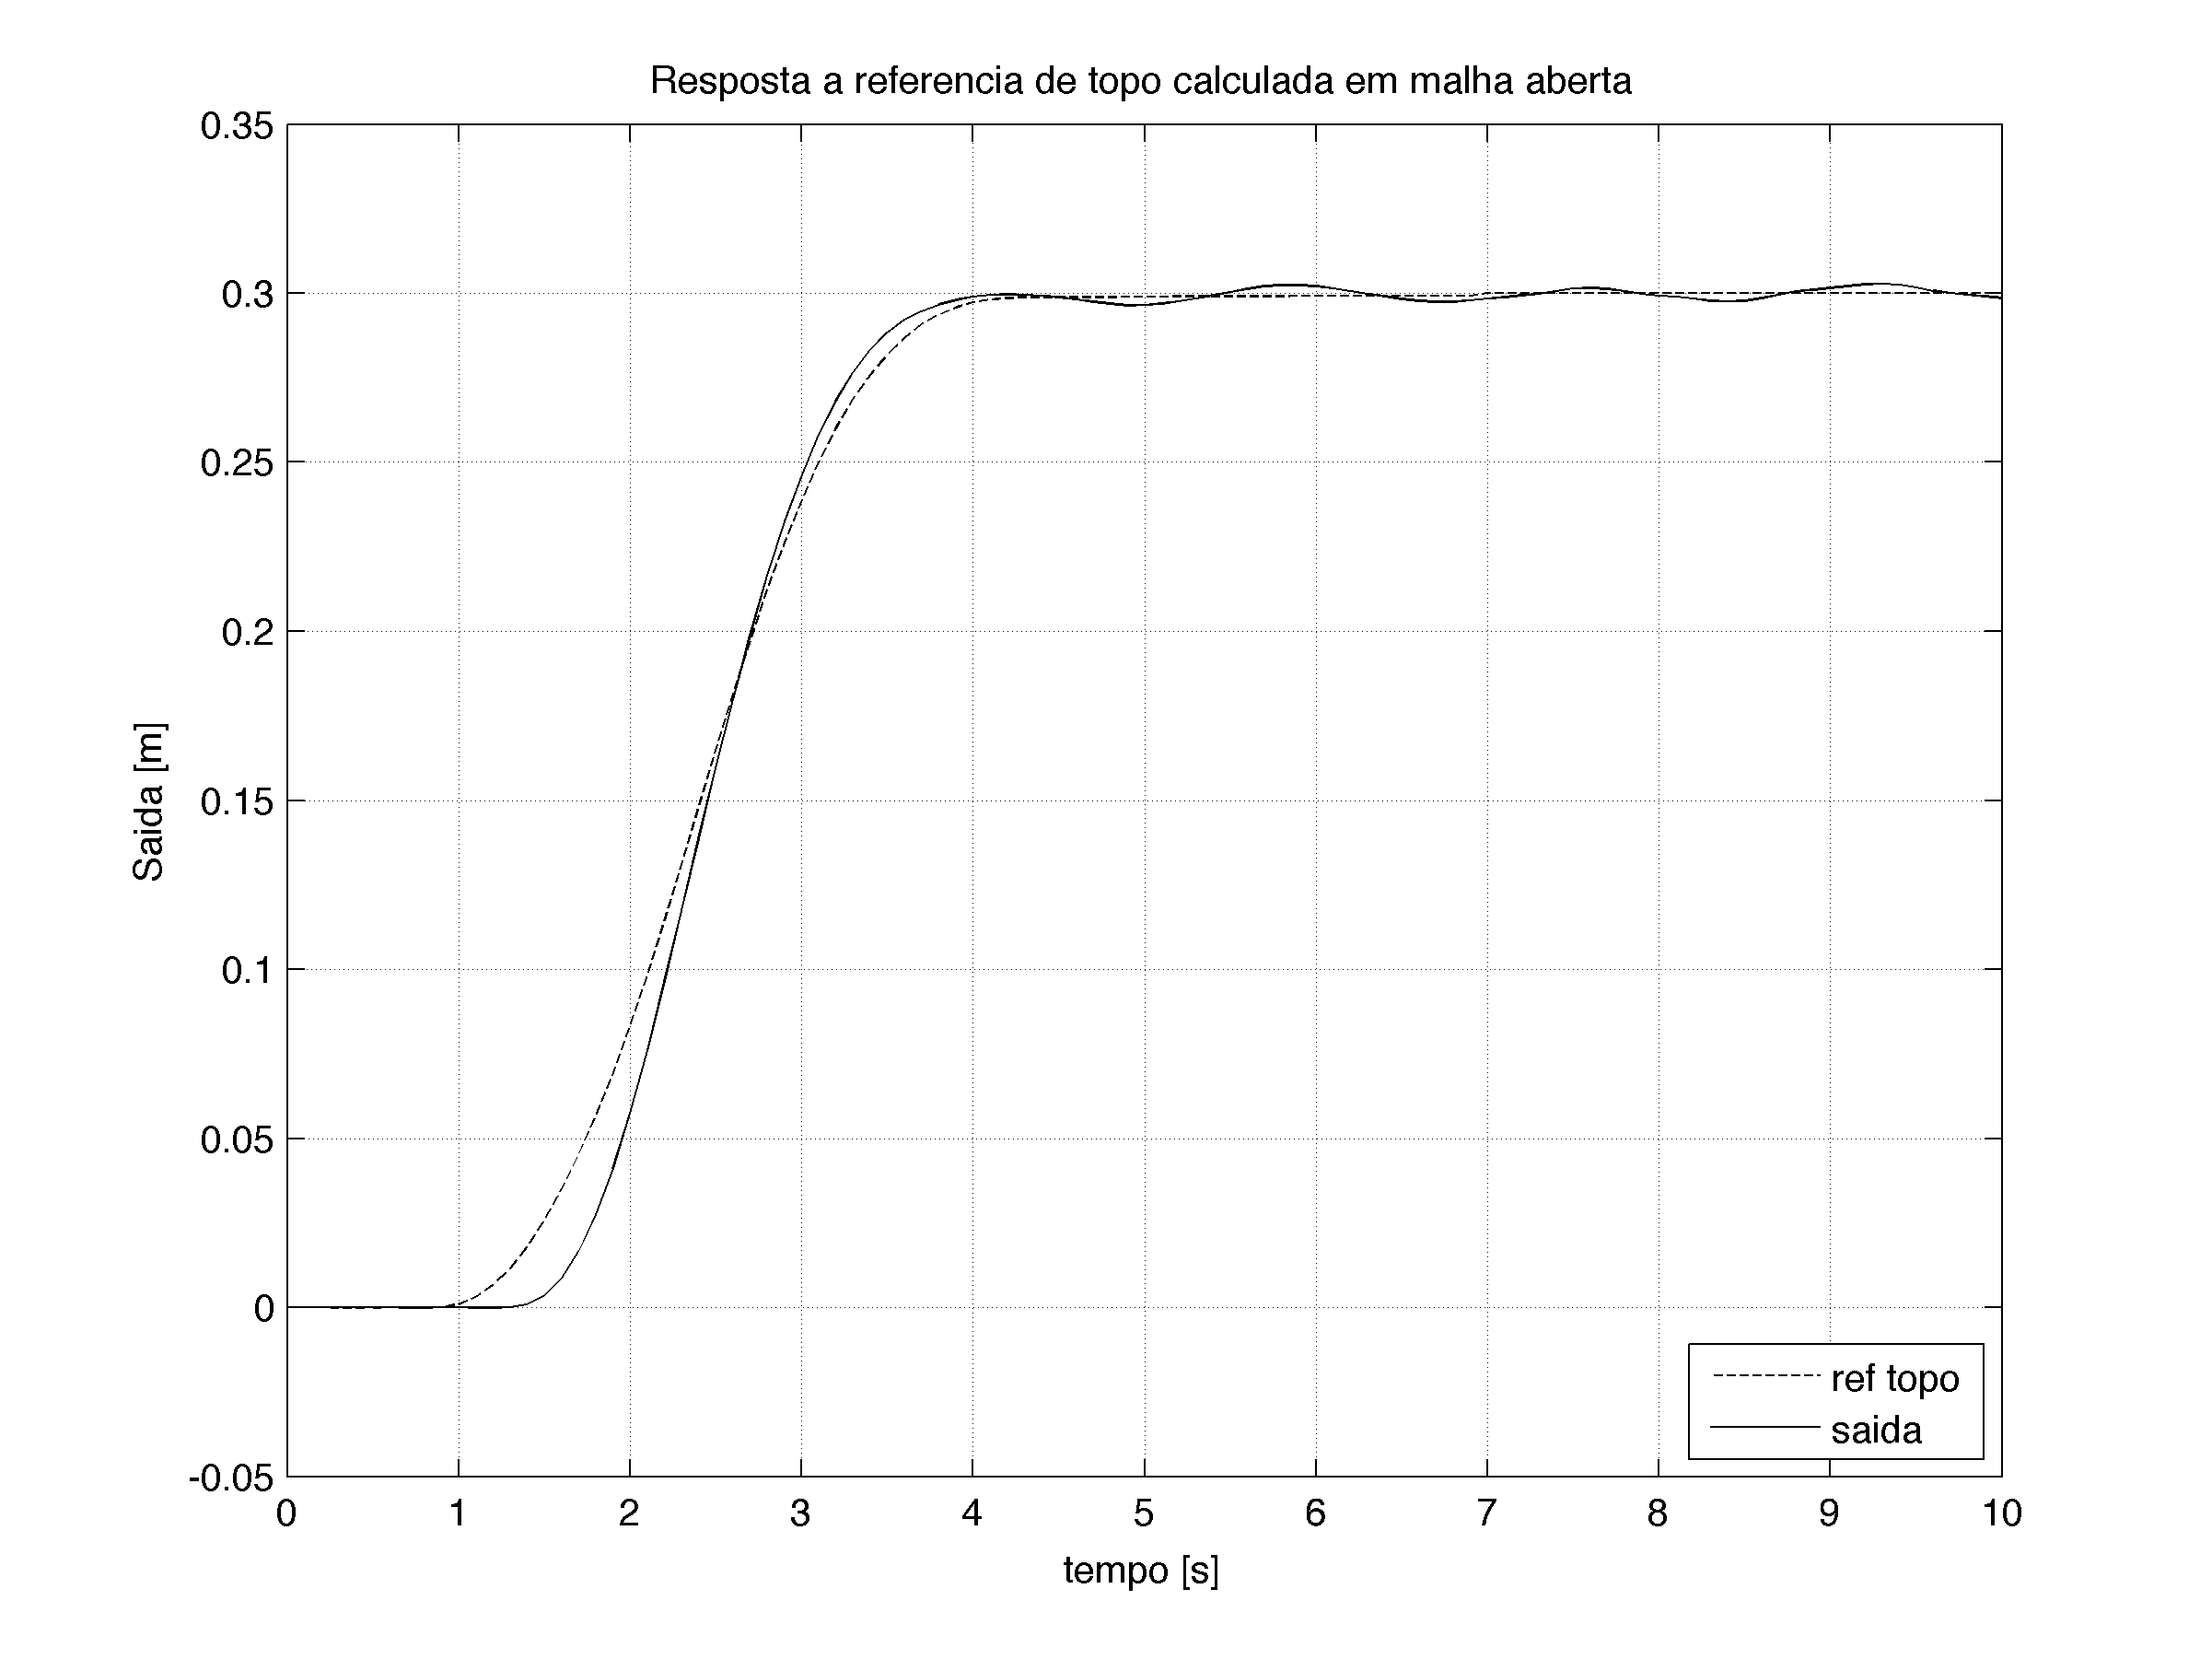
\includegraphics[width=1\linewidth]{figs/resultados/simulacao/respostaMalhaAbertaRefTopo}
        \caption{Resposta do Sistema em Malha Aberta para Excursão de 30cm, entrada suave calculada\label{respostaMalhaAbertaEntradaSuave}}
    \end{minipage}
\end{figure}

 A solução para lidar com perturbações é fechar a malha. Para isso, uma vez obtidos os ganhos, Equação \ref{ganhosObtidos}, fez-se o projeto do sistema em malha fechada em Simulink \cite{simulink}. A Figura \ref{topModel} apresenta os principais blocos e suas conexões. Nos somadores, as referências para a posição de topo, que é a posição do carrinho, e para a posição de fundo, que é a posição da bolinha, são as entradas do sistema. O bloco \texttt{PLANTA} é o modelo sem redução modal. No caso deste projeto, a matriz do sistema sem redução de ordem é de dimensão $400\times 400$. Os blocos \texttt{Signal Builder} representam um sinal tipo rampa definido para comparação com as trajetórias suaves de topo e fundo \cite{rafaelMestrado}. 
 

\begin{figure}[!ht]
\centering

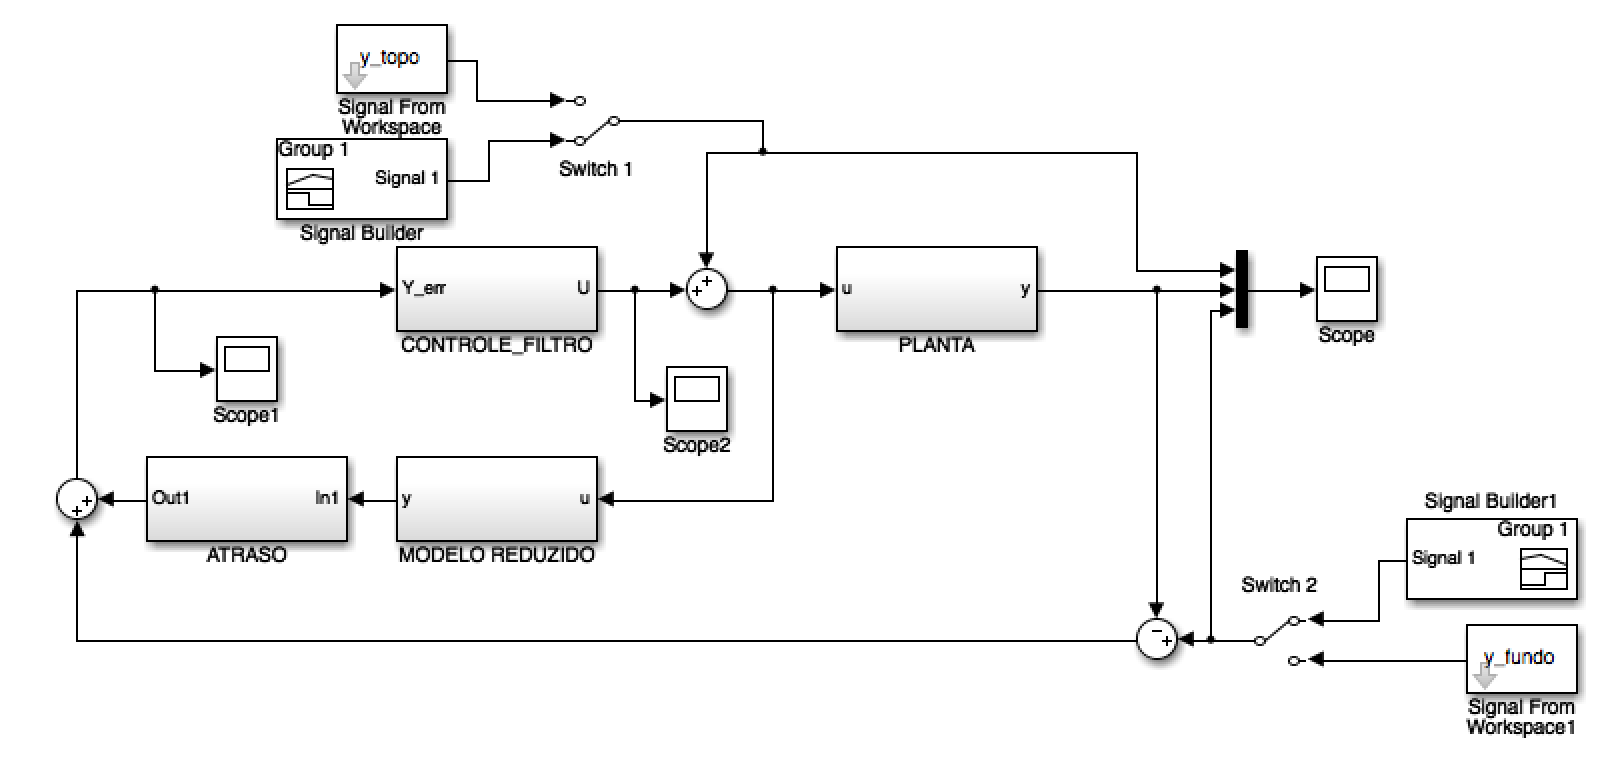
\includegraphics[width=0.9\linewidth]{figs/resultados/simulink/top}
\caption{Esquema principal para simulação em Simulink\label{topModel}}
\end{figure}

 O bloco atraso, Figura \ref{blocoAtraso}, tem como saída o valor predito pelo modelo reduzido menos esse mesmo sinal atrasado em 3 períodos de amostragem, uma vez que $\epsilon \simeq 3T_s$. Esse valor é somado à diferença entre a referência de fundo e a saída da planta para então ser a entrada do bloco de controle. O bloco \texttt{CONTROLE\_FILTRO} é detalhado na Figura \ref{blocoControle} e utiliza os ganhos da Equação \ref{ganhosObtidos}. O filtro de Kalman utilizou, como matrizes de covariância, $Q = 0.01^2 I_4$ e $R = 0.4^2$; tais valores foram obtidos de forma empírica.

\begin{figure}[!ht]
\centering

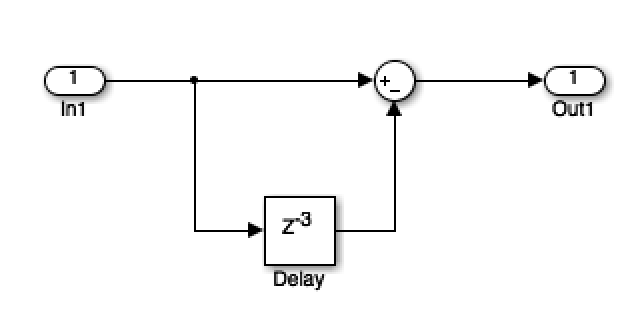
\includegraphics[width=0.5\linewidth]{figs/resultados/simulink/atraso}
\caption{Bloco de Atraso -- saída é o valor antecipado menos um valor antigo\label{blocoAtraso}}
\end{figure}

\begin{figure}[!ht]
\centering

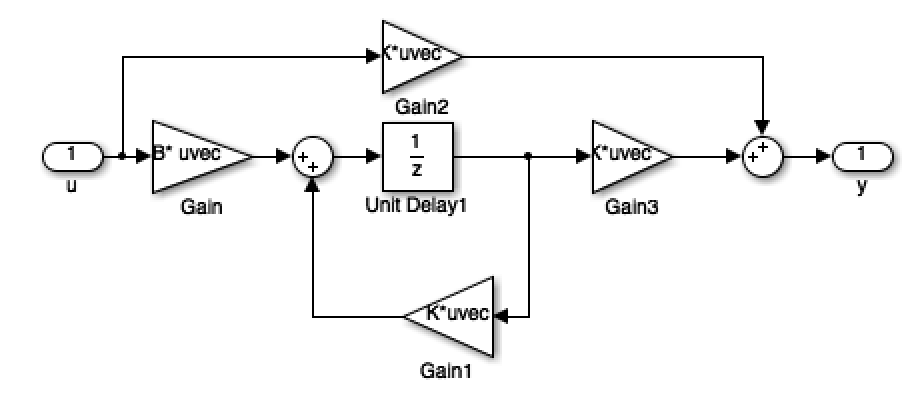
\includegraphics[width=0.6\linewidth]{figs/resultados/simulink/modeloReduzido}
\caption{Modelo reduzido -- não utiliza atraso, utilizado para predizer a saída\label{blocoModeloReduzido}}
\end{figure}

\begin{figure}[!ht]
\centering
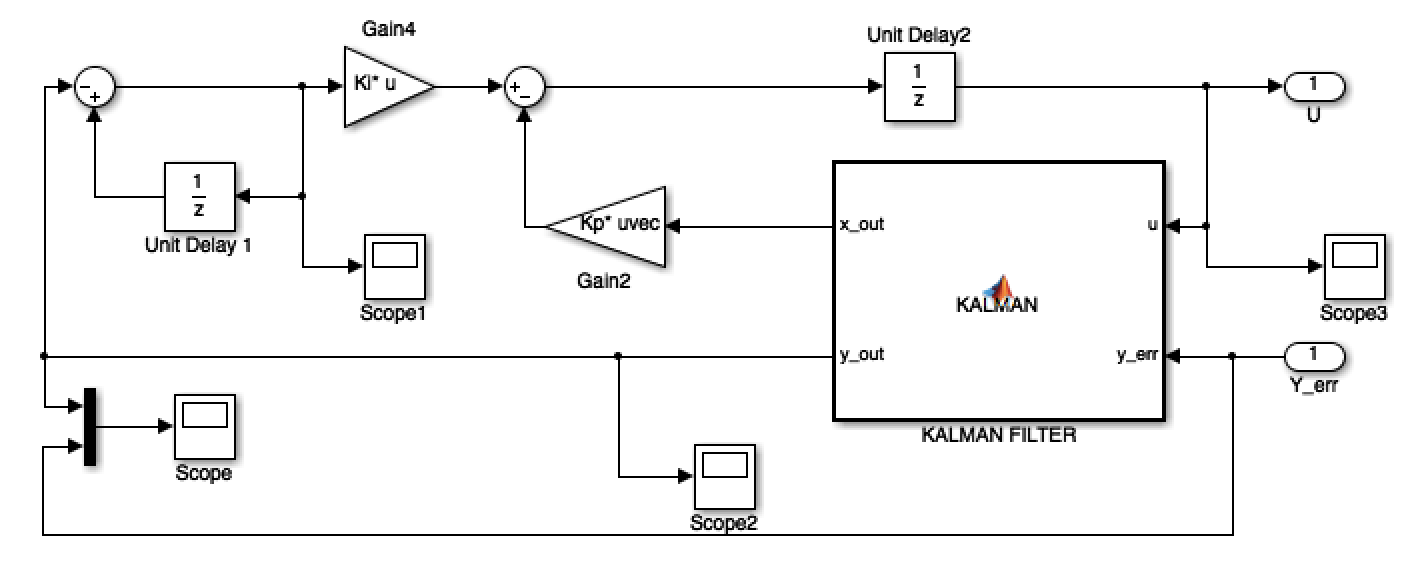
\includegraphics[width=0.9\linewidth]{figs/resultados/simulink/controle}
\caption{Bloco de controle com filtro de Kalman\label{blocoControle}}

\end{figure}

 O resultado das simulações sem ruído é apresentado nas Figuras \ref{respostaMalhaFechadaRampa} e \ref{respostaMalhaFechadaRefTopoFundo}. Nota-se uma ótima melhoria na resposta à rampa, enquanto a resposta à entrada suave se mantém boa.


\begin{figure}[!htb]
    \centering
    \begin{minipage}{.45\textwidth}
        \centering
       
        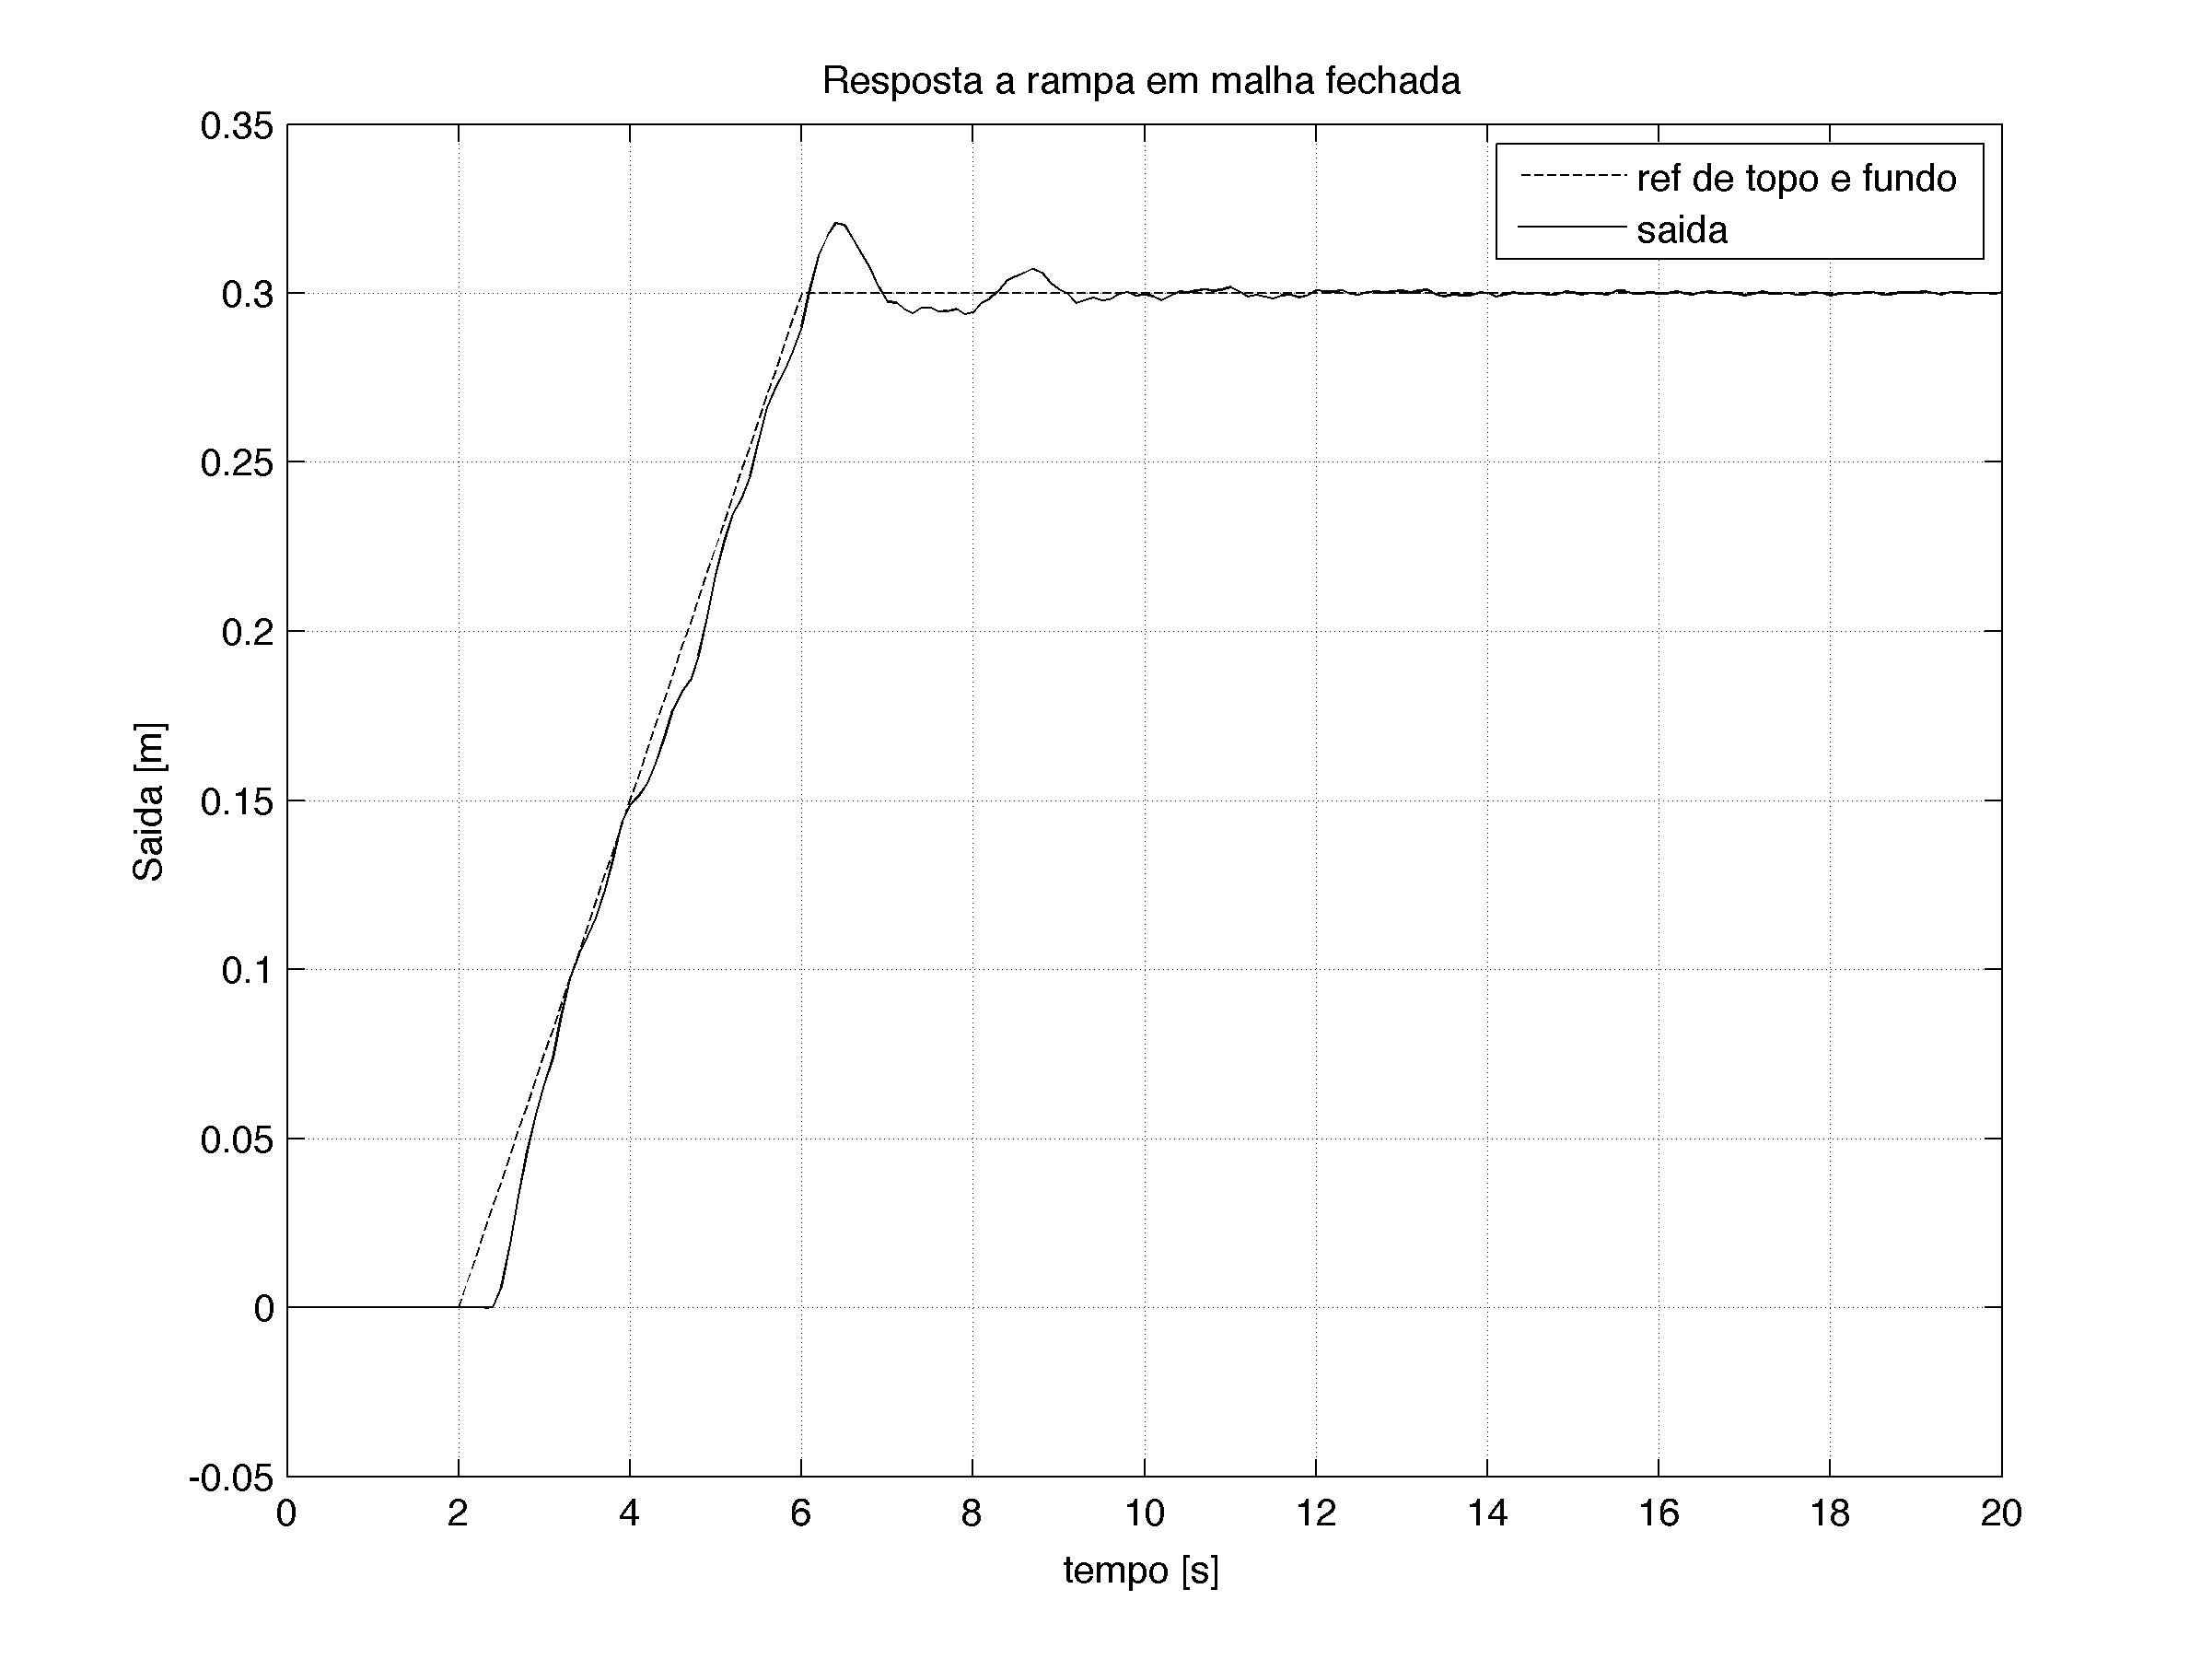
\includegraphics[width=1\linewidth]{figs/resultados/simulacao/respostaMalhaFechadaRampa}
        \label{respostaMalhaFechadaRampa}
         \caption{Resposta do Sistema em Malha Fechada para Excursão de 30cm, entrada rampa}
    \end{minipage}%
    \hspace{0.1cm}
    \begin{minipage}{0.45\textwidth}
        \centering
      
        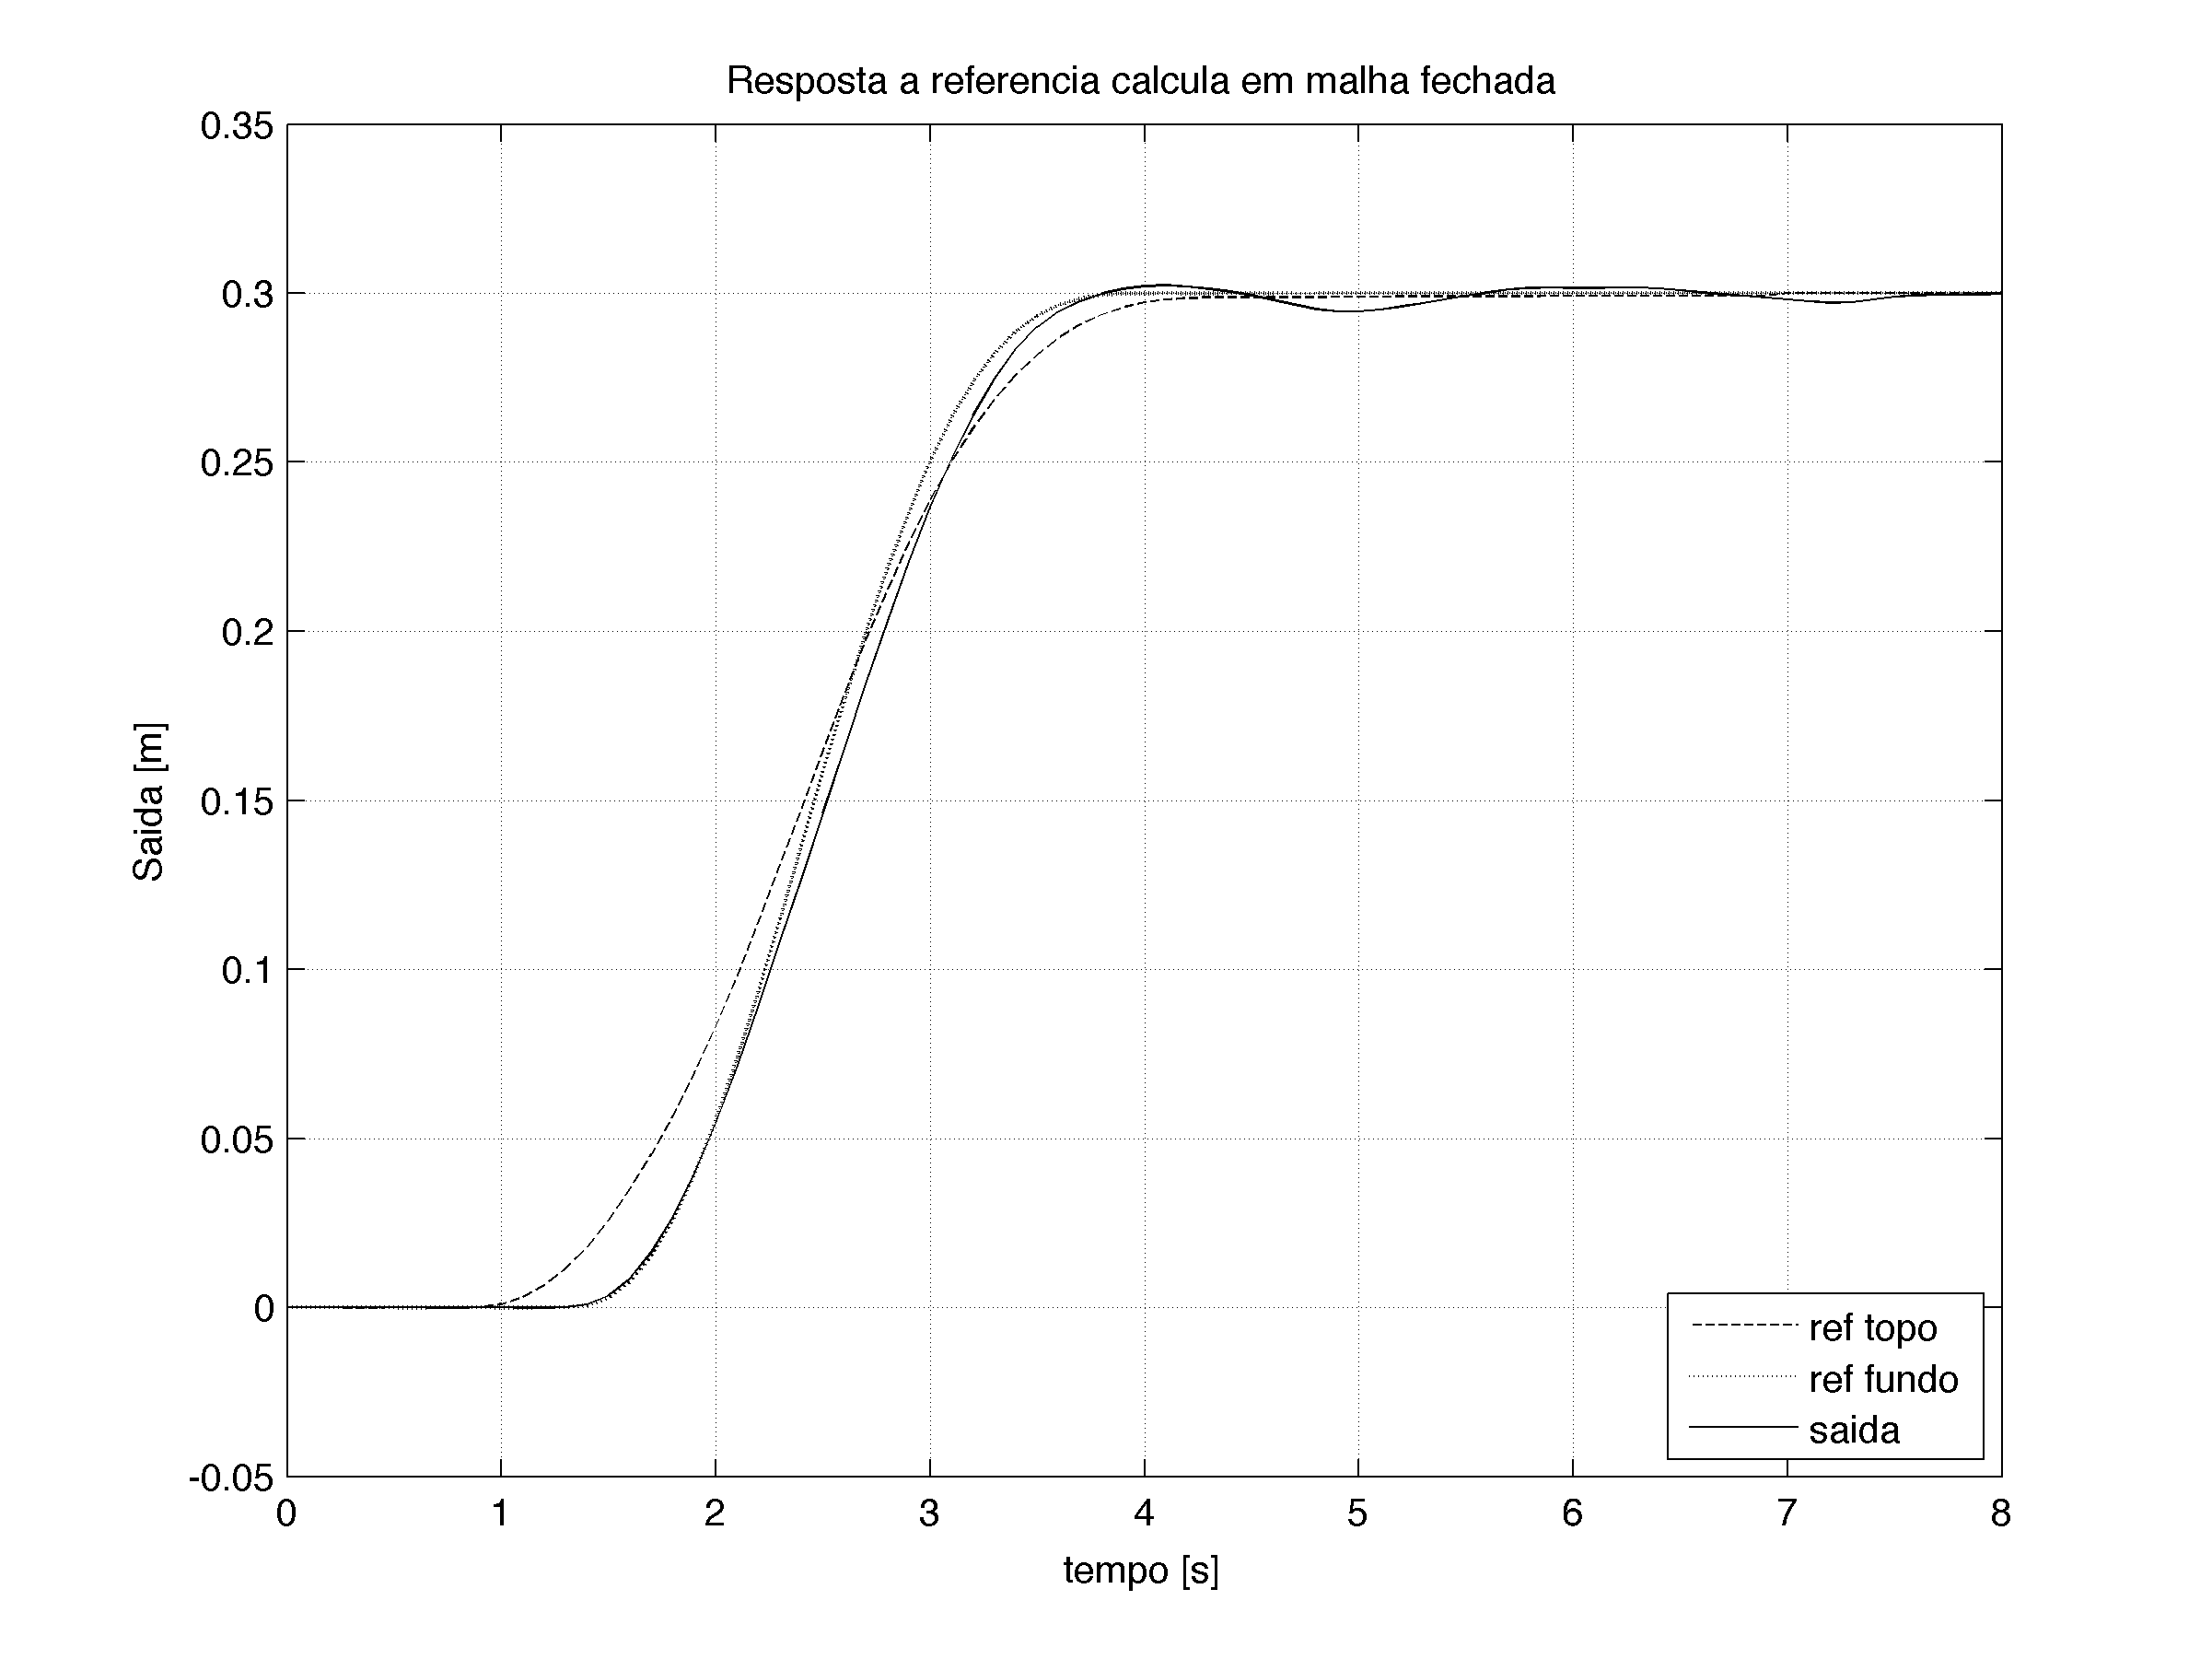
\includegraphics[width=1\linewidth]{figs/resultados/simulacao/respostaMalhaFechadaRefTopoFundo}
        \label{respostaMalhaFechadaRefTopoFundo}
        \caption{Resposta do Sistema em Malha Fechada para Excursão de 30cm, entrada suave calculada para topo e fundo}
    \end{minipage}
\end{figure}

Algo essencial é analisar a resistência ao ruído. Ela depende não só da malha fechada, mas também do filtro de Kalman que foi implementado. Os parâmetros $Q$ e $R$ escolhidos anteriormente são essenciais para uma boa atenuação de ruídos. O ruído foi inserido na simulação conforme a Figura \ref{simulacaoComRuidoSimulink}. O que se nota é que o sinal de entrada do bloco de controle sempre terá algum erro, o que seria um erro no sistema de medição. O resultado da simulação é apresentado na Figura \ref{respostaMalhaAbertaRefTopoRuido}. É importante observar a diferença entre o sinal de referência antes e depois de ser somado o ruído. Conforme a Figura \ref{entradaControladorYERR} apresenta, esse sinal tem grandes variações comparado ao original; mesmo assim, o resultado final está bem controlado, evidenciando a importância do controle em malha fechada com a presença do Filtro de Kalman como observador. 

\begin{figure}[!ht]
\centering

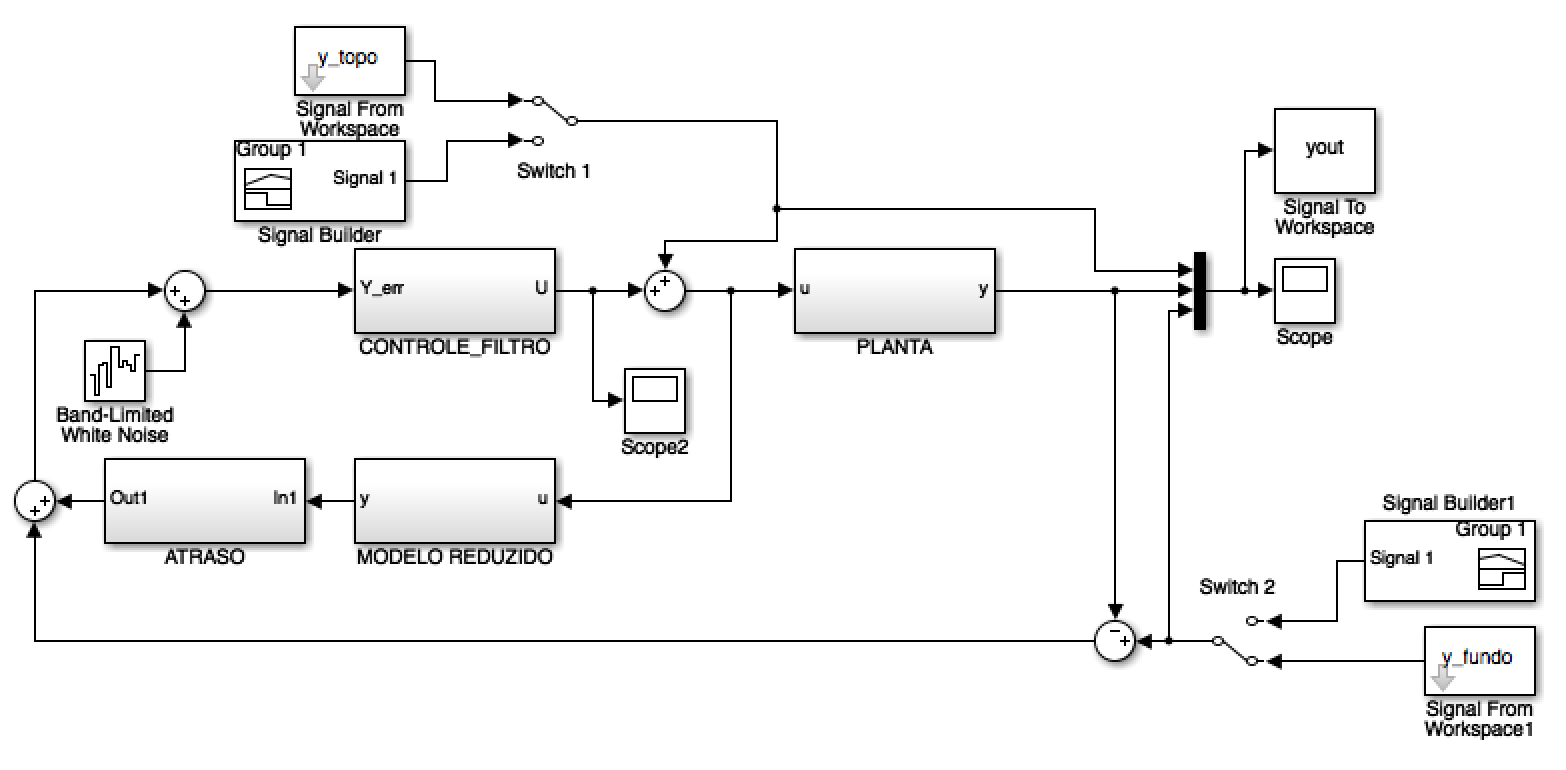
\includegraphics[width=0.8\linewidth]{figs/resultados/simulacao/simulacaoComRuido}
\caption{Sistema com um ruído branco adicionado\label{simulacaoComRuidoSimulink}}
\end{figure}


\begin{figure}[!htb]
    \centering
    \begin{minipage}{.45\textwidth}
        \centering
        
        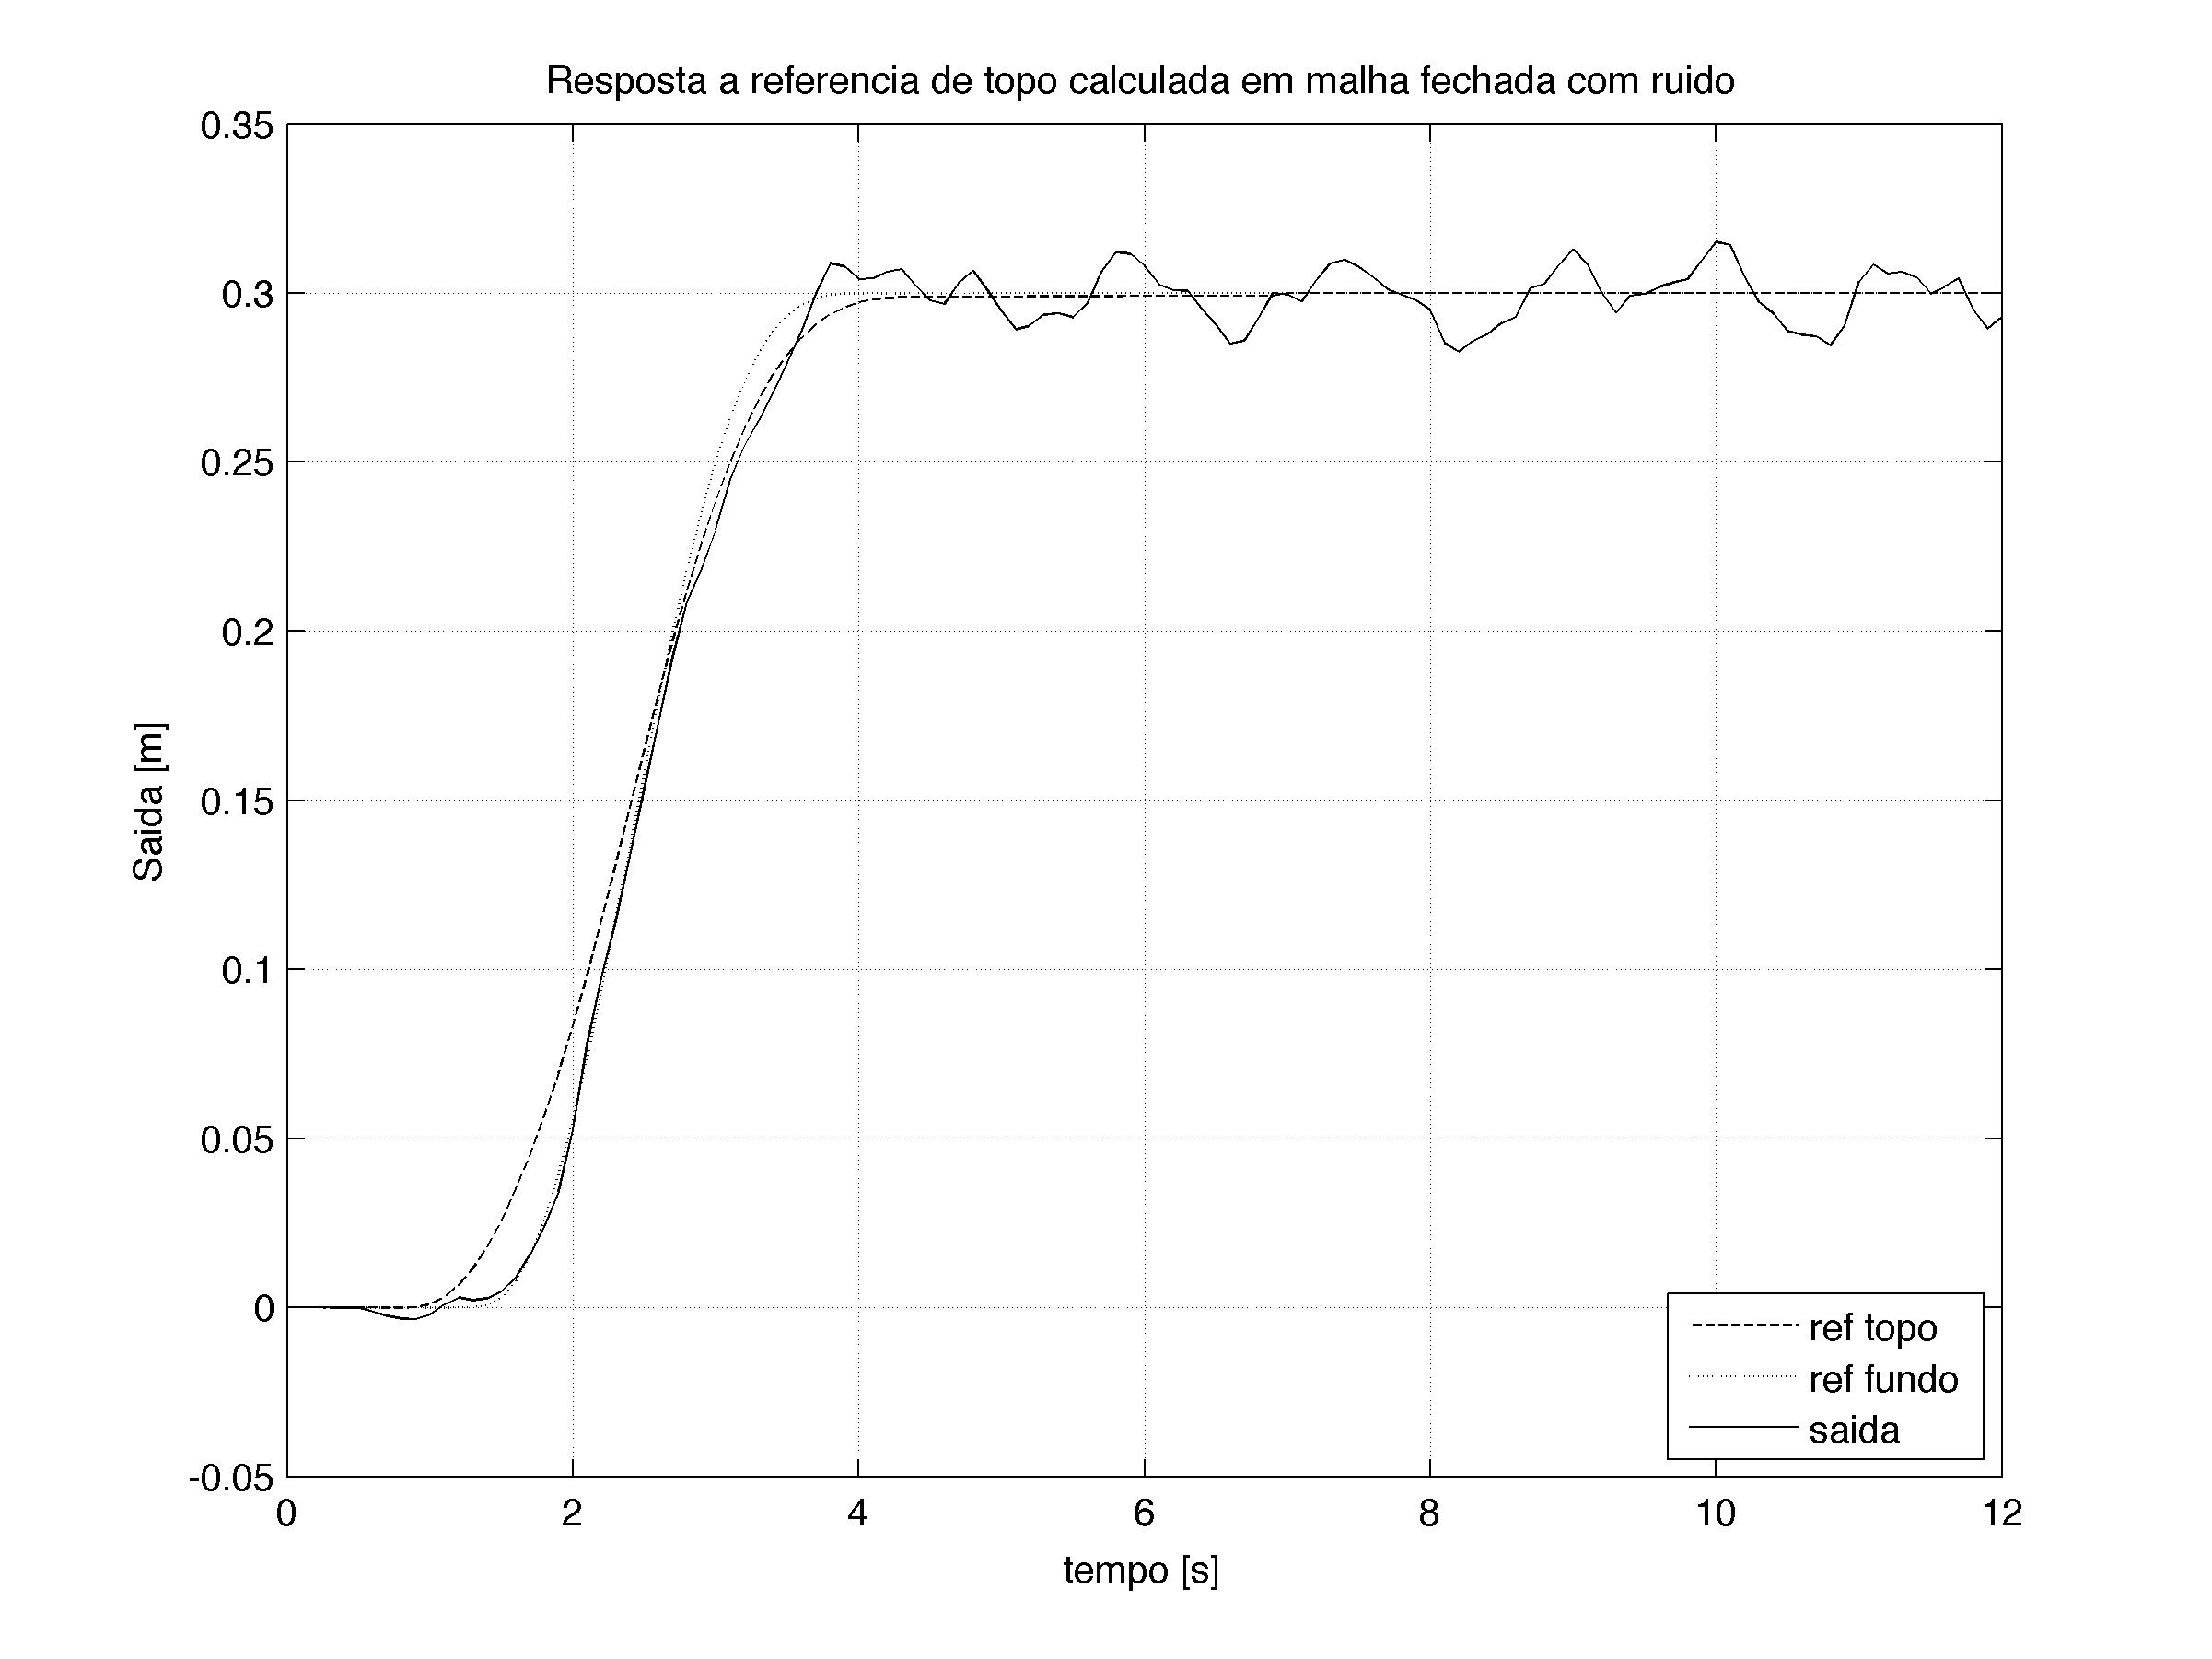
\includegraphics[width=1\linewidth]{figs/resultados/simulacao/respostaMalhaAbertaRefTopoRuido}
        \caption{Resposta do Sistema em Malha Fechada para Excursão de 30cm, entrada suave, com ruído\label{respostaMalhaAbertaRefTopoRuido}}
    \end{minipage}%
    \hspace{0.1cm}
    \begin{minipage}{0.45\textwidth}
        \centering
               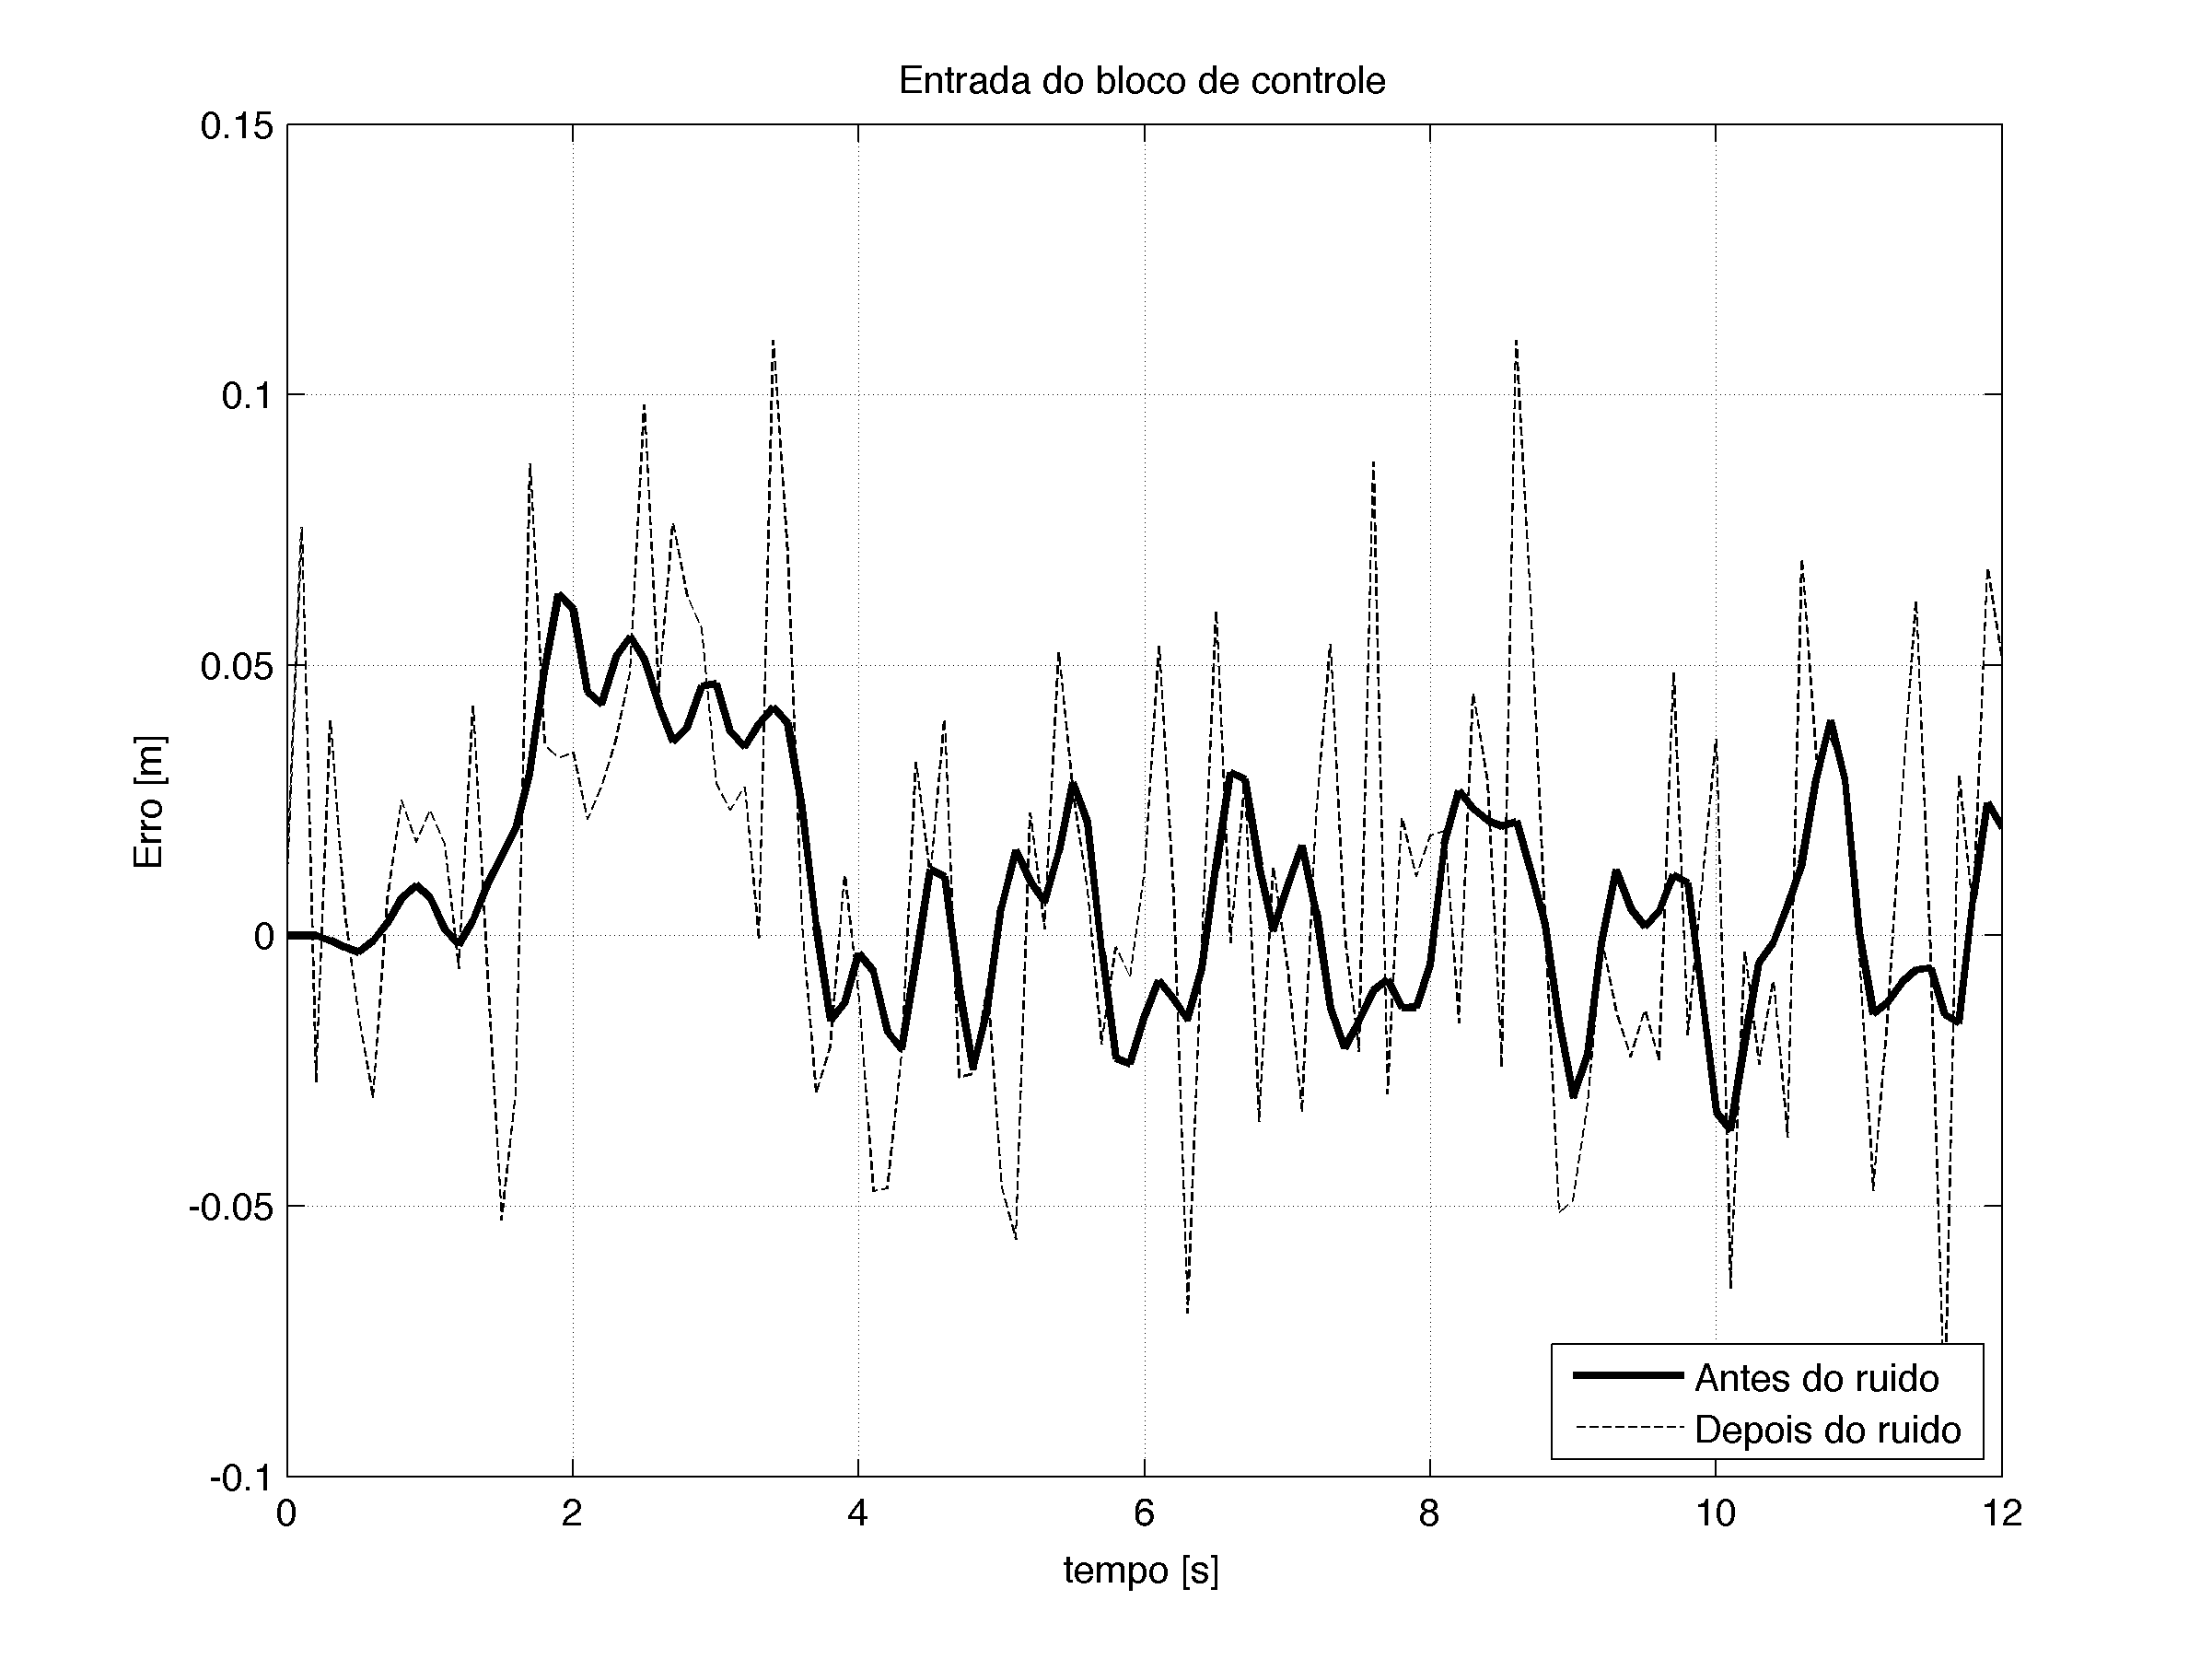
\includegraphics[width=1\linewidth]{figs/resultados/simulacao/entradaControladorYERR}
        \caption{Entrada do controlador antes e depois do ruído para cada instante\label{entradaControladorYERR}}

    \end{minipage}
\end{figure}


\section{Resultados Experimentais}
\subsection{Considerações Iniciais}
De posse das simulações feitas, assumindo-se que o sistema se comporta de forma estável e desejada com os polos escolhidos e as matrizes de covariância obtidas para o Filtro de Kalman, prosseguiu-se com a validação experimental do controle proposto. Para tal, em conjunção com os programas necessários desenvolvidos no RSLogix, foram desenvolvidos módulos e códigos em linguagem Python para implementar o controle. As três principais razões de se utilizar Python são:
\begin{enumerate}
\item A linguagem Python, conforme discutido na Seção \ref{opcSubSection}, possui suporte ao módulo OpenOPC \cite{OpenOPC}, necessário para se efetuar a troca de informações entre o preditor de Smith e a planta por intermédio do CLP;
\item Embora haja outras linguagens e \textit{softwares} que suportem OPC, como o próprio MATLAB, além de existirem linguagens mais rápidas e ao mesmo tempo ricas em ferramentas como o C++, o uso de Python se deve ao fato de já ter o módulo OPC e ser razoavelmente rápido, talvez não tanto quanto o C++. Porém, dada a facilidade de se programar com o OpenOPC e os tempos de comunicação e execução dos programas feitos não interferirem com o tempo de amostragem, Python se torna uma opção extremamente viável para este projeto;
\item Além do módulo OpenOPC, facilidade de programação e tempos razoáveis, Python possui também suporte à orientação a objetos. Para programar estruturas como o preditor de Smith, tal abordagem é muito importante, visto que cada componente pode ser tratado como um objeto, facilitando a implementação. Além disso, a estrutura de programação é tal que outras formas de controle podem ser facilmente adaptadas à ponte rolante por meio da interface com Python; as alterações no programa do RSLogix são mínimas, caso sejam necessárias.
\end{enumerate}

Assim como nas simulações, foram considerados três experimentos a serem validados: trajetória em malha aberta; trajetória em malha fechada, considerando topo e fundo como rampas; e a trajetória considerada por Rafael \cite{rafaelMestrado}. Todas as trajetórias consideram excursão de 30 centímetros.

\subsection{Testes com Rampa - Malha Aberta e Malha Fechada}
O primeiro teste feito foi considerando uma trajetória em formato rampa, realizando um deslocamento de 30 centímetros em cerca de 2.5 segundos. Tal teste foi feito em malha aberta\footnote{Teste Experimental com Rampa em Malha Aberta --- \url{https://youtu.be/chrez0QEucU}. Acesso em 30/06/2016.} e o resultado se encontra na Figura \ref{malhaAbertaRampa}. 

O segundo teste realizado considerou a mesma trajetória do primeiro teste como referência tanto para o topo quanto para o fundo para um experimento com a malha fechada, utilizando-se o preditor de Smith\footnote{Teste Experimental com Rampa utilizando Preditor de Smith --- \url{https://youtu.be/QOuxlsT3gBA}. Acesso em 30/06/2016.}. O resultado se encontra na Figura \ref{malhaFechadaRampa}.

\begin{figure}[!ht]
\centering
\begin{minipage}{0.45\textwidth}
\centering
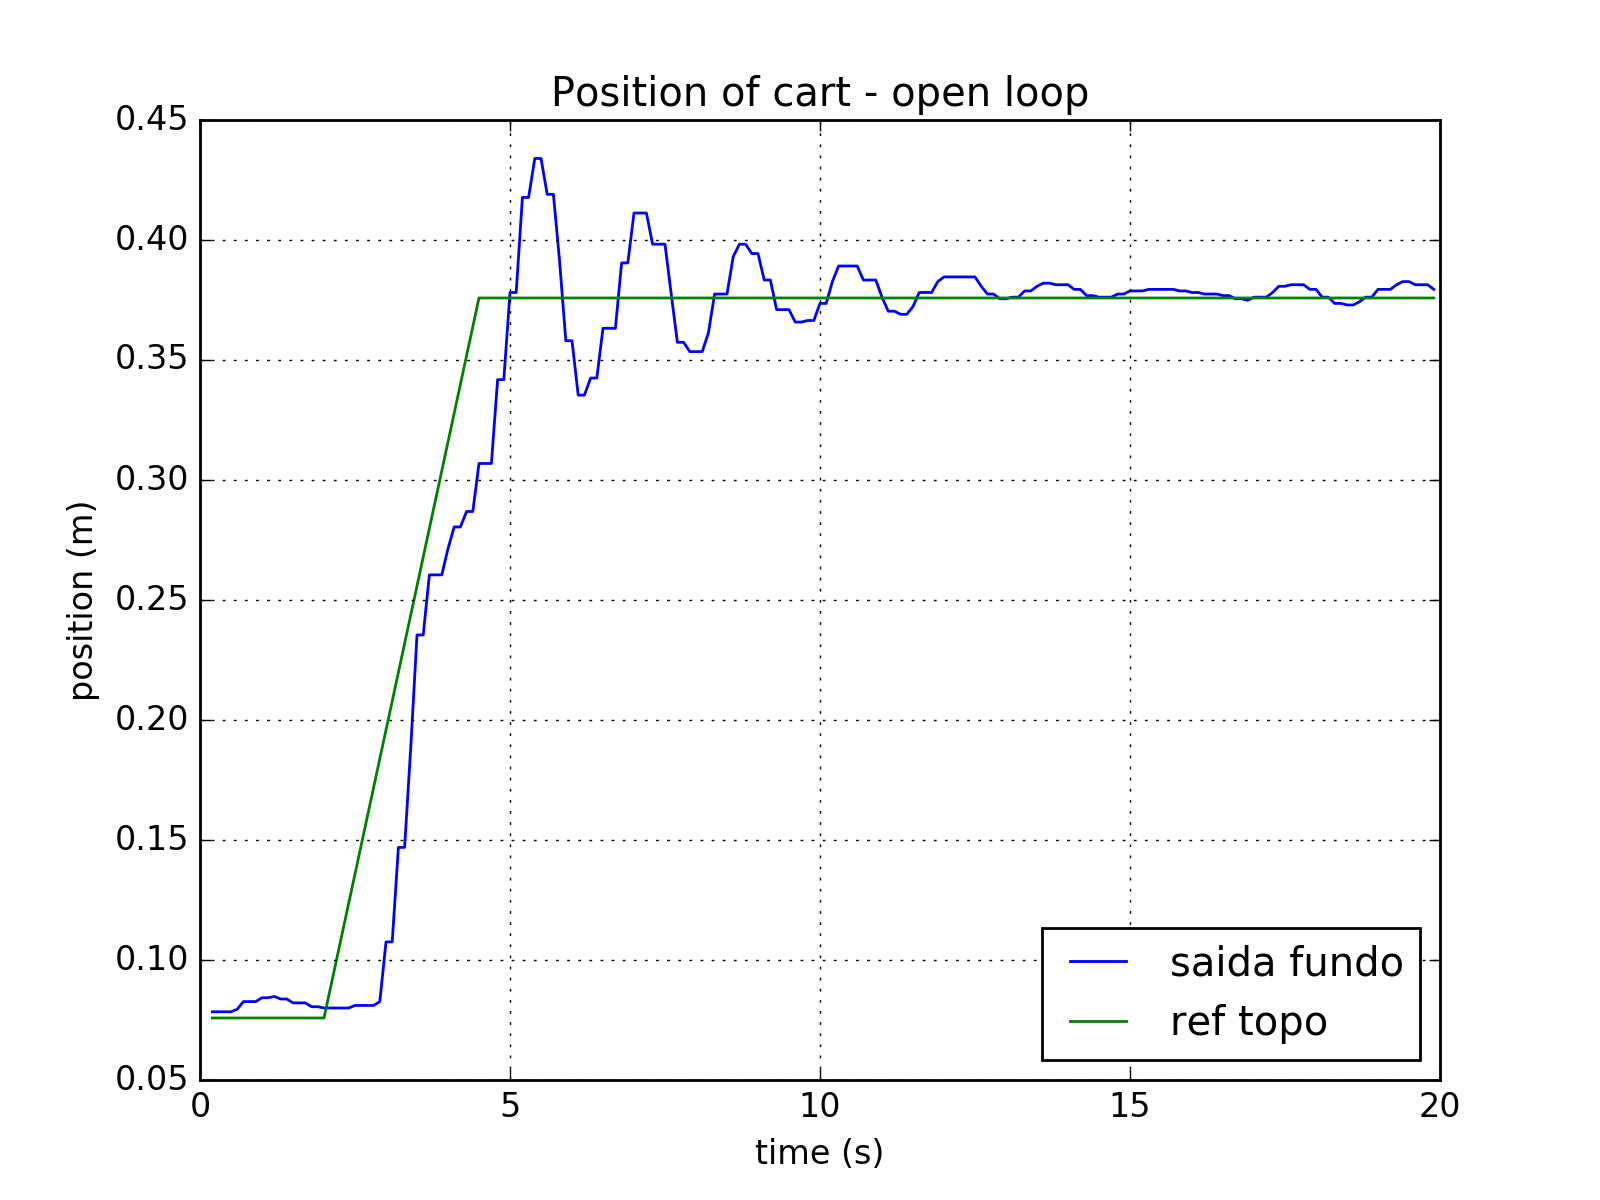
\includegraphics[width=1\linewidth]{figs/resultados/experimento/open_loop_ramp}
\caption{Resultado experimental para a trajetória rampa em malha aberta de 30 cm. \label{malhaAbertaRampa}}
\end{minipage}
\hspace{0.1cm}
\begin{minipage}{0.45\textwidth}
\centering
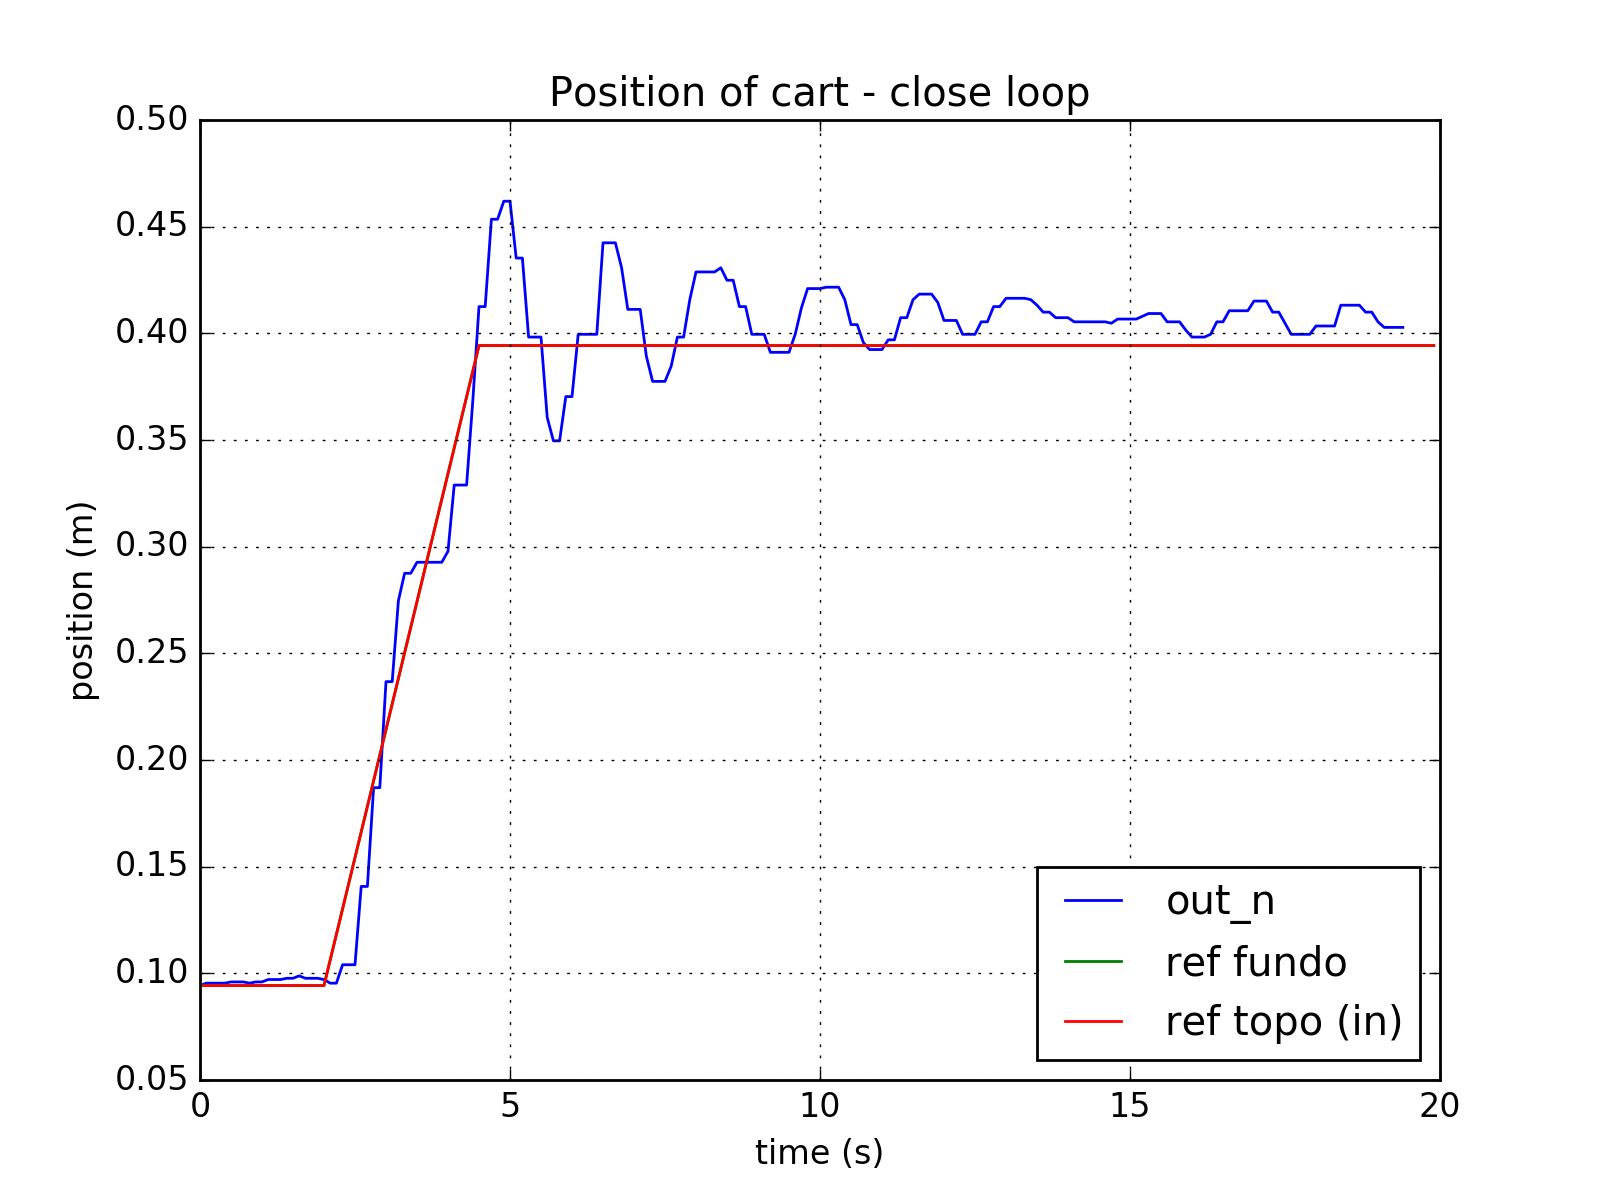
\includegraphics[width=1\linewidth]{figs/resultados/experimento/closed_loop_trajetoria_rampa}
\caption{Resultado experimental para a trajetória rampa em malha fechada de 30 cm. \label{malhaFechadaRampa}}
\end{minipage}
\end{figure}

Nota-se, pelos resultados apresentados, que cada um dos testes realizados com a rampa possuem vantagens e desvantagens entre si: a trajetória em malha aberta apresentou um sobressinal ligeiramente menor e melhor aproximação com o resultado final; entretanto, a trajetória em malha fechada foi melhor seguida durante o movimento. Em termos práticos, considerando a presente trajetória, o preditor de Smith realizou melhor a tarefa do acompanhamento da trajetória, mas o controle em malha fechada deixou a desejar, já que as oscilações não foram controladas. A Figura \ref{rampaComparativo} mostra os dois resultados comparados em um mesmo gráfico, subtraindo-se a posição inicial de cada teste.

\begin{figure}[!ht]
\centering
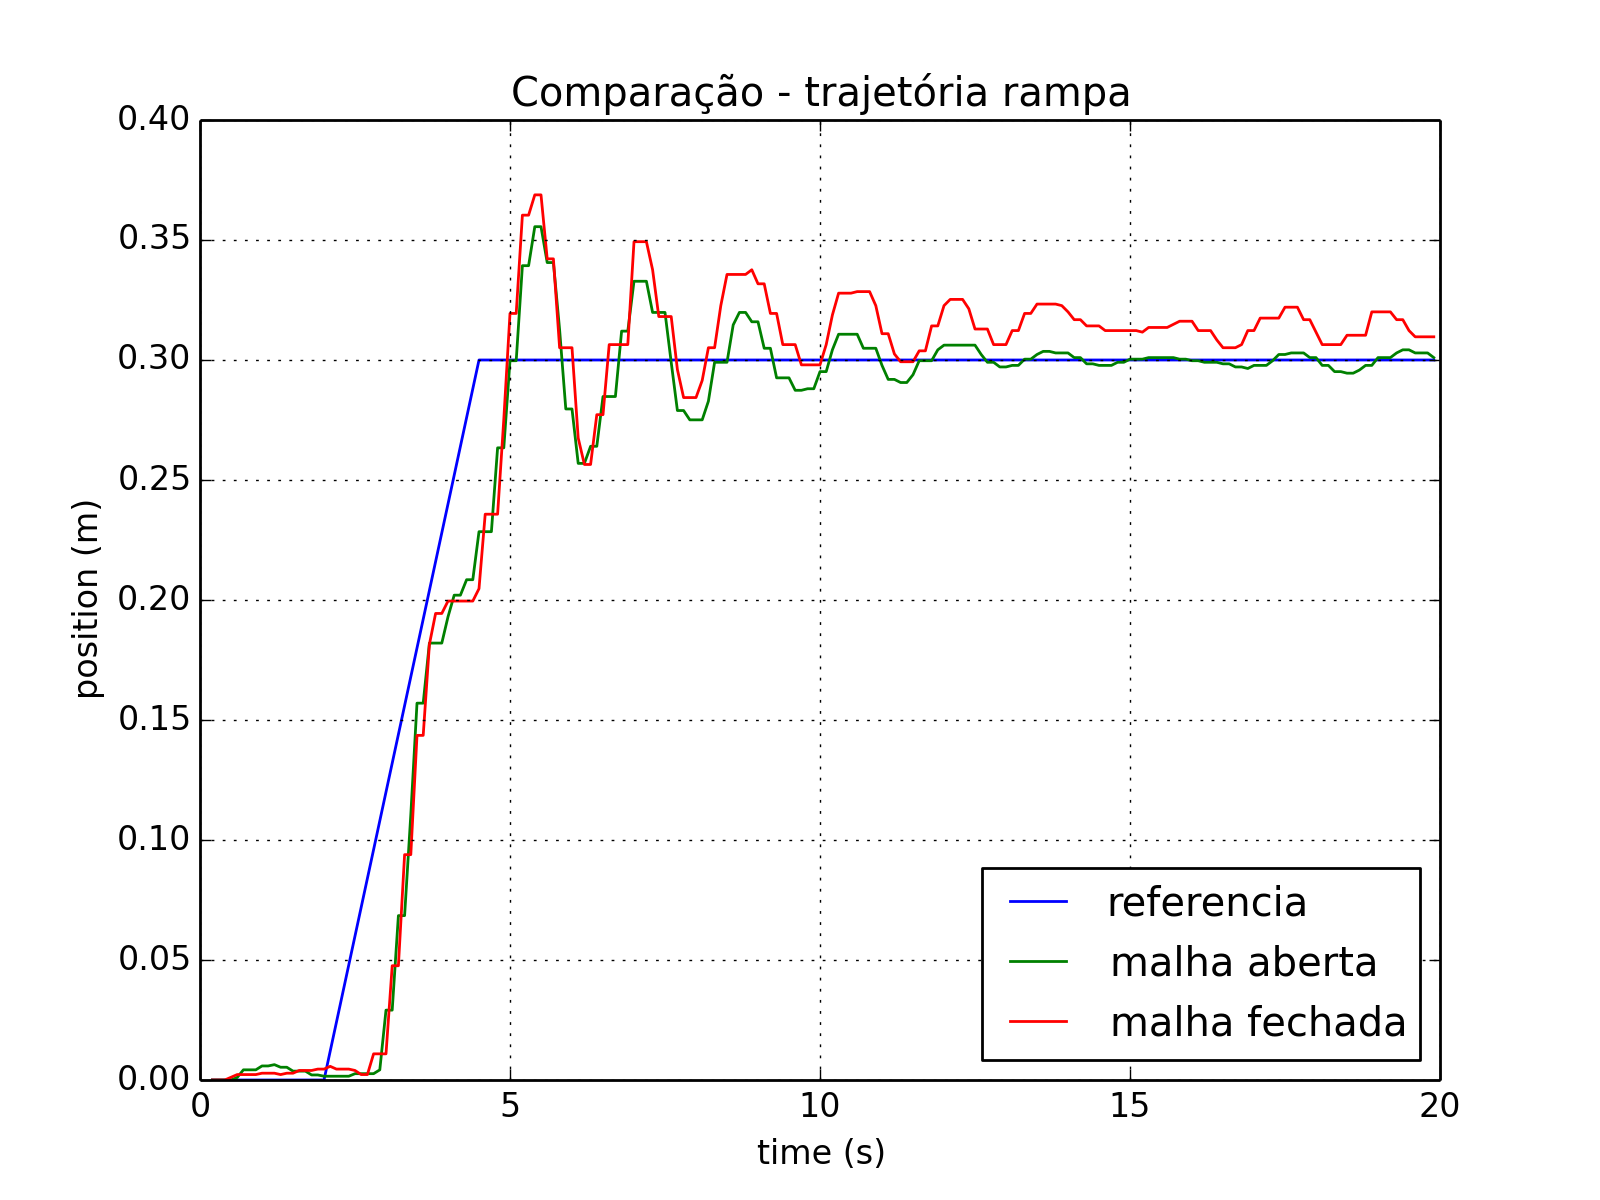
\includegraphics[width=.6\linewidth]{figs/resultados/experimento/rampa_comp}
\caption{Gráfico comparativo das respostas em malha aberta e malha fechada com trajetória rampa. \label{rampaComparativo}}
\end{figure} 

Motivos para o resultado ruim, ainda mais se comparado com o experimental na Figura \ref{malhaFechadaRampa}, incluem erros de calibração -- a câmera é desconfigurada rapidamente no laboratório de automação -- e o fato de termos utilizado OPC adicionava um atraso na comunicação para fechar a malha e às vezes o próximo valor medido não era lido rápido o suficiente para ser considerado no próximo passo de simulação. O filtro de Kalman possivelmente pode ter parâmetros melhores escolhidos com mais alguns testes experimentais, o que poderia também melhorar problemas com ruído.

\subsection{Teste com Trajetória Proposta - Malha Fechada}
O último teste realizado com o preditor de Smith envolve a trajetória utilizada por Rafael \cite{rafaelMestrado}. Nesse caso, a trajetória de topo e de fundo são ligeiramente diferentes, sugerindo uma trajetória próxima do esperado para um \textit{riser}. O resultado do experimento\footnote{Teste Experimental com Trajetória Proposta por Rafael\cite{rafaelMestrado} utilizando Preditor de Smith --- \url{https://youtu.be/lpPZ7HOG7hM}. Acesso em 30/06/2016.} se encontra na Figura \ref{experimentoRafael}. Nota-se que a saída é bem comportada, seguindo a trajetória; porém, o resultado final apresenta pequenas oscilações, além de um erro de medição. A Figura \ref{experimentoRafaelDetalhe} mostra em detalhe a saída, durante o tempo em que a trajetória é executada. 

\begin{figure}[!ht]
\centering
\begin{minipage}{.45\textwidth}
\centering
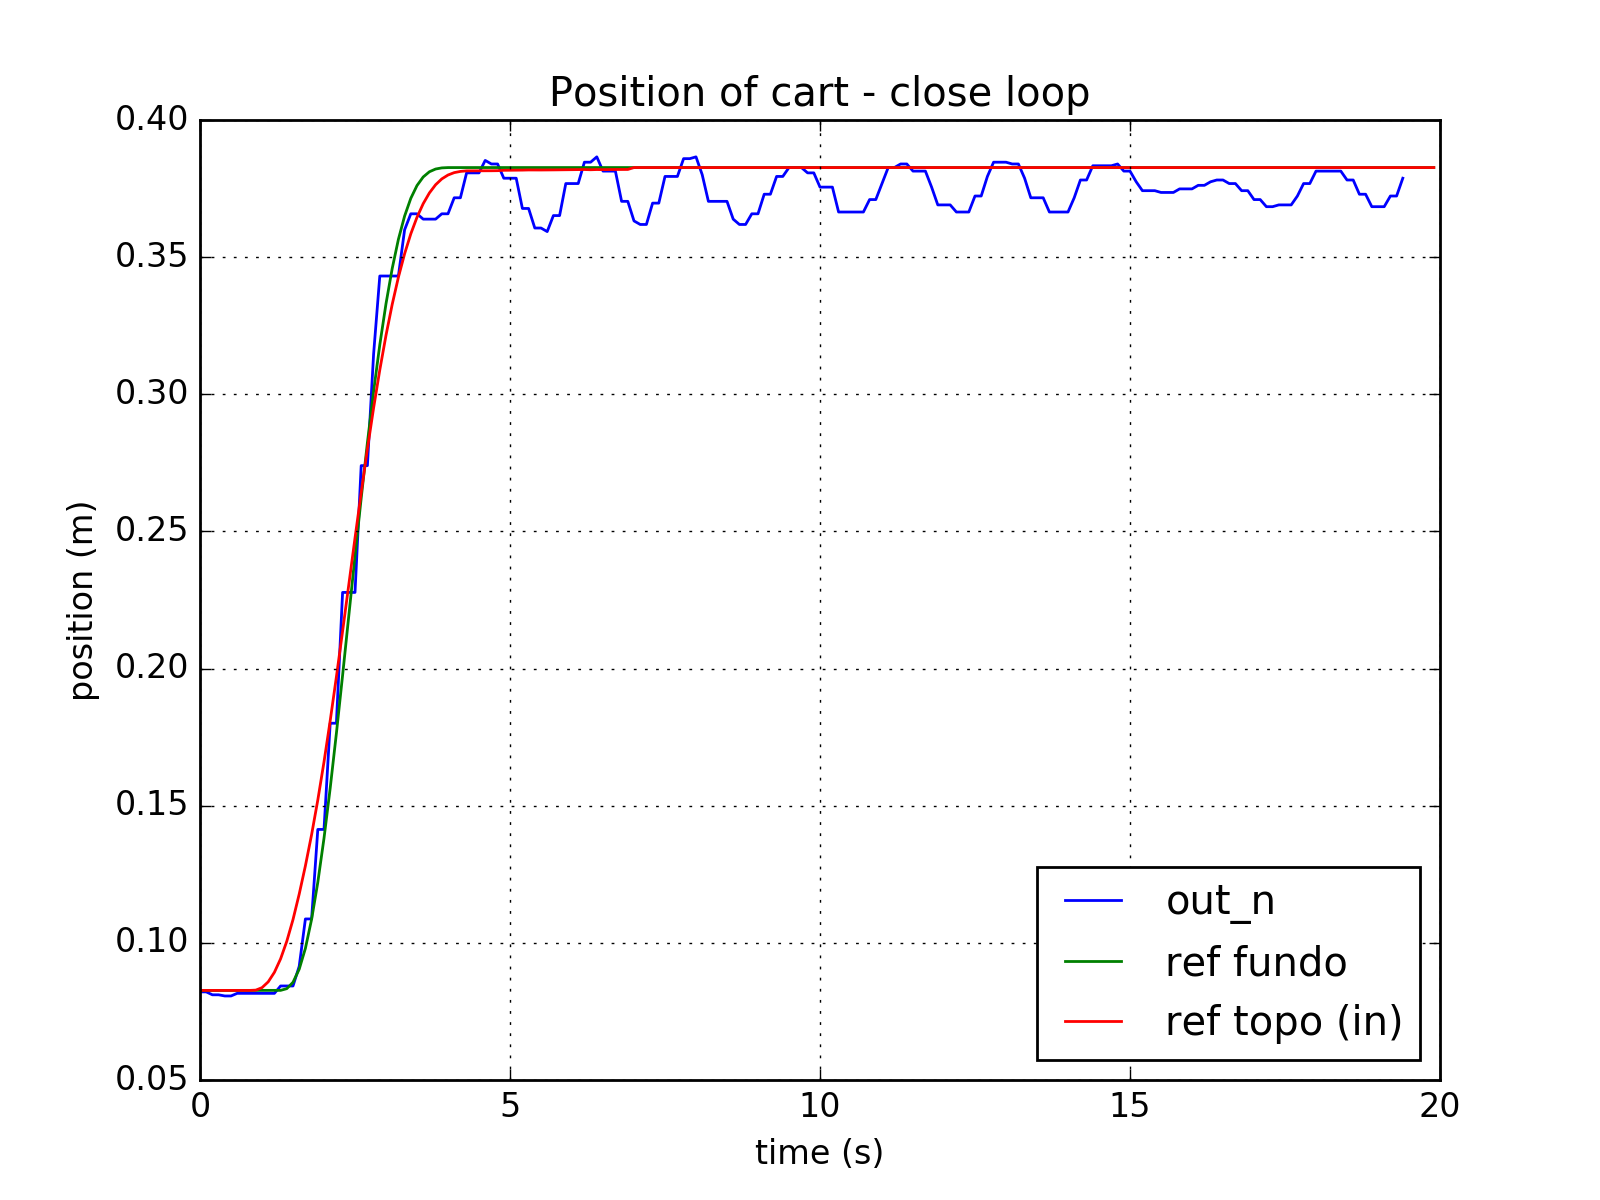
\includegraphics[width=1\textwidth]{figs/resultados/experimento/closed_loop_trajetoria_rafael}
\caption{Teste com a trajetória sugerida por Rafael utilizando o preditor de Smith. \label{experimentoRafael}}
\end{minipage}
\hspace{0.1cm}
\begin{minipage}{.45\textwidth}
\centering
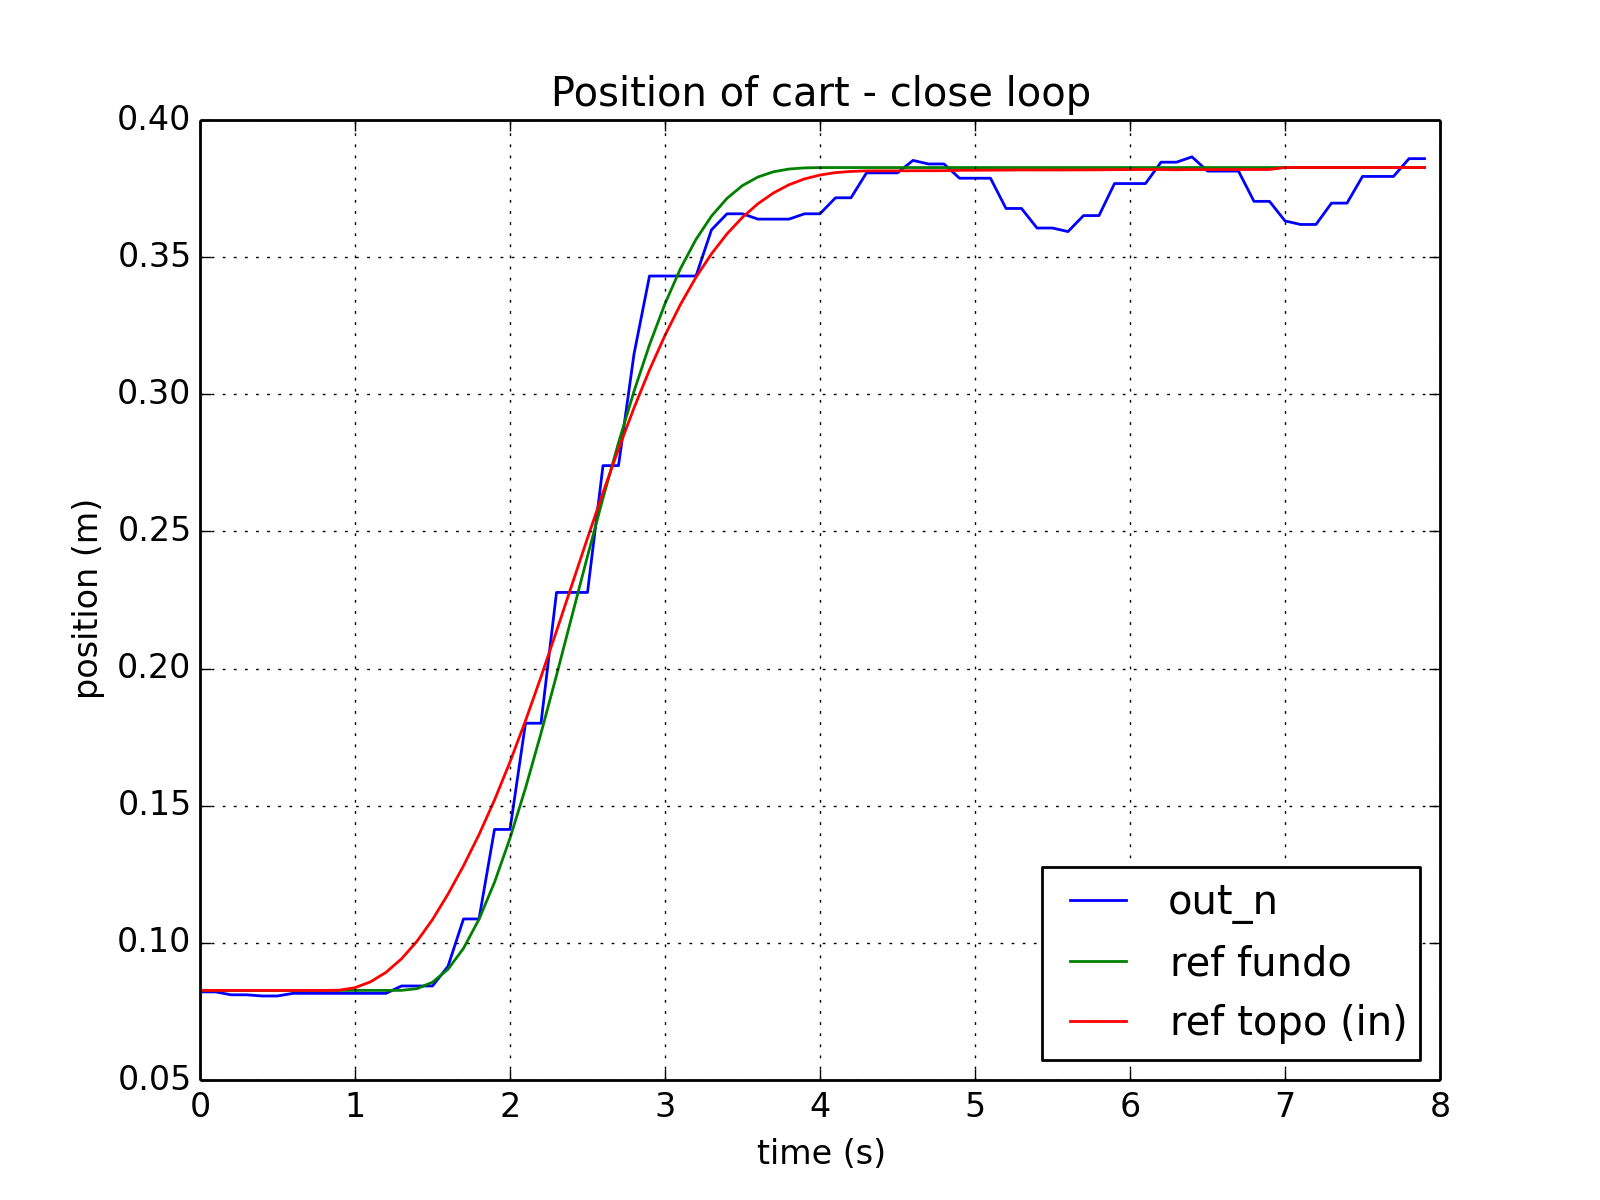
\includegraphics[width=1\textwidth]{figs/resultados/experimento/closed_loop_trajetoria_rafael_detalhe}
\caption{Teste com a trajetória sugerida por Rafael, detalhando a execução da trajetória. \label{experimentoRafaelDetalhe}}
\end{minipage}
\end{figure} 

Deve-se notar que houveram alguns resultados indesejáveis nos testes apresentados, em particular os que envolvem o preditor. Em primeiro lugar, houve a presença de um sobressinal considerável nos testes com rampa -- cerca de $12.5\%$. Esse tipo de sobressinal pode ser extremamente prejudicial para a operação do \textit{riser}. Além do problema do sobressinal, houve o fato de que a saída oscila e apresenta um erro estático nos testes com o preditor, representados nas Figuras \ref{malhaFechadaRampa} e \ref{experimentoRafael}; embora a presença desses fatores faz o resultado experimental destoar dos resultados das simulações, o resultado geral foi satisfatório. Um resultado marcante foi a atenuação da saída proporcionado pelo uso do Filtro de Kalman, considerando as matrizes de covariância escolhidas; o fato da matriz $\mathbf{R}$ possuir valores maiores do que os elementos de $\mathbf{Q}$ sugere que foi priorizada a correção sobre a medida da posição de fundo.